\documentclass[12pt,                   
               a4paper,                 
               twoside,                 
               openright,               
               italian,
               article]{book}   
\usepackage[Lenny]{fncychap}
\usepackage{array} 
\newcolumntype{L}{>{\centering\arraybackslash}m{3cm}}
\usepackage{wrapfig}
\usepackage{cite}
\usepackage{color}
\usepackage{adjustbox}
\usepackage{multirow}
\usepackage{subcaption}
\usepackage{float}
\usepackage{amsmath,amssymb,amsthm}    % matematica
\usepackage[T1]{fontenc}  
\usepackage[utf8]{inputenc}             % codifica di input; anche [latin1] va bene
\usepackage[italian]{babel}    % per scrivere in italiano e in inglese;

%\usepackage{bookmark}                   % segnalibri
\usepackage{caption}                    % didascalie
\usepackage{csquotes}                   % gestisce automaticamente i caratteri (")
\usepackage{commath}
\usepackage{arrayjobx}
\usepackage{emptypage}                  % pagine vuote senza testatina e piede di pagina

\usepackage{epigraph}			% per epigrafi

\usepackage{eurosym}                    % simbolo dell'euro

%\usepackage{indentfirst}               % rientra il primo paragrafo di ogni sezione

\usepackage{graphicx}                   % immagini

\usepackage{lscape}

\usepackage{tocbibind}

%\usepackage{hyperref}                   % collegamenti ipertestuali

%\usepackage[binding=5mm]{layaureo}      % margini ottimizzati per l'A4; rilegatura di 5 mm

\usepackage{listings}                   % codici

\usepackage{microtype}                  % microtipografia

\usepackage{mparhack,fixltx2e,relsize}  % finezze tipografiche

\usepackage{nameref}                    % visualizza nome dei riferimenti                                      

\usepackage[font=small]{quoting}        % citazioni

\usepackage[italian]{varioref}          % riferimenti completi della pagina

\usepackage[dvipsnames]{xcolor}         % colori

\usepackage{booktabs}                   % tabelle                                       
\usepackage{tabularx}                   % tabelle di larghezza prefissata                                    
\usepackage{longtable}                  % tabelle su più pagine                                        
\usepackage{ltxtable}                   % tabelle su più pagine e adattabili in larghezza
\usepackage{imakeidx}
\usepackage{hyperref}
\makeindex[columns=2, options= -s index_style.ist, intoc]

\newcommand{\RN}[1]{%
  \textup{\uppercase\expandafter{\romannumeral#1}}%
}

%\usepackage[acronym]{glossaries}
% Generate the glossary
%\makeglossaries

%\newglossaryentry{glsy}
%{
%    name=glossary,
%    description={Acronyms and terms which are generally unknown or new to common readers.}
%}
%\newacronym{kd}{KD}{Knowledge Distillation}

%\usepackage[acronym]{glossaries}   % glossario
                                        % per includerlo nel documento bisogna:
                                        % 1. compilare una prima volta tesi.tex;
                                        % 2. eseguire: makeindex -s tesi.ist -t tesi.glg -o tesi.gls tesi.glo
                                        % 3. eseguire: makeindex -s tesi.ist -t tesi.alg -o tesi.acr tesi.acn
                                        % 4. compilare due volte tesi.tex.
%\makeglossaries
%\newacronym{gcd}{GCD}{Greatest Common Divisor}
%\setcounter{tocdepth}{3}
%\setcounter{secnumdepth}{3}

\captionsetup[figure]{labelsep=period}
\captionsetup[subfigure]{labelformat=simple} % default is 'parens'
\renewcommand\thesubfigure{\thefigure.\alph{subfigure}.}
\DeclareMathOperator*{\argmax}{argmax}
\DeclareMathOperator*{\argmin}{argmin}
\newtheorem{corollary}{CorollaURry}

%**************************************************************
% SETTINGS
%************************************************************** 
%**************************************************************
% file contenente le impostazioni della tesi
%**************************************************************

%**************************************************************
% Frontespizio
%**************************************************************

% Autore
\newcommand{\myName}{Flavio Forenza}                                    

%\HRule \\ [0.4cm] % Horizontal line
\newcommand{\myTitle}{Distilled-Single-Shot-Detector (DSSD): un nuovo modello di guida autonoma ad alta inferenza}
%\HRule \\ [1.5cm] % Horizontal line

% Università             
\newcommand{\myUni}{UNIVERSITÀ DEGLI STUDI DI MILANO}

% Dipartimento
\newcommand{\myDepartment}{DIPARTIMENTO DI INFORMATICA GIOVANNI DEGLI ANTONI}

% Facoltà       
\newcommand{\myFaculty}{\emph{Corso di Laurea Magistrale in Informatica}}

% Titolo del relatore
\newcommand{\profTitle}{Prof.}
\newcommand{\correlatoreTitle}{Dott.}

% Relatore
\newcommand{\myProf}{Vincenzo Piuri}
\newcommand{\myCorrelatore}{Angelo Genovese}

% Luogo
\newcommand{\myLocation}{Milano}

% Anno accademico
\newcommand{\myAA}{2020/2021}

% Data discussione
\newcommand{\myTime}{...}


%**************************************************************
% Impostazioni di impaginazione
% see: http://wwwcdf.pd.infn.it/AppuntiLinux/a2547.htm
%**************************************************************

\setlength{\parindent}{14pt}   % larghezza rientro della prima riga
\setlength{\parskip}{0pt}   % distanza tra i paragrafi
\renewcommand{\baselinestretch}{1.5}

%**************************************************************

\usepackage{float} %per inserire figure in mezzo al testo

\usepackage{listings} % per inserire codice 

\usepackage{afterpage}
\newcommand\blankpage{
    \null
    \thispagestyle{empty}
    \addtocounter{page}{+1}
    \newpage
    }

%**************************************************************
% Impostazioni di caption
%**************************************************************
\captionsetup{
    tableposition=top,
    figureposition=bottom,
    font=small,
    format=hang,
    labelfont=bf
}

%**************************************************************
% Impostazioni di glossaries
%**************************************************************
%\input{glossario} % database di termini
%\makeglossaries


%**************************************************************
% Impostazioni di graphicx
%**************************************************************
\graphicspath{{images/}} % cartella dove sono riposte le immagini


%**************************************************************
% Impostazioni di hyperref
%**************************************************************
\hypersetup{
    %hyperfootnotes=false,
    %pdfpagelabels,
    %draft,	% = elimina tutti i link (utile per stampe in bianco e nero)
    colorlinks=true,
    linktocpage=true,
    pdfstartpage=1,
    pdfstartview=FitV,
    % decommenta la riga seguente per avere link in nero (per esempio per la stampa in bianco e nero)
    %colorlinks=false, linktocpage=false, pdfborder={0 0 0}, pdfstartpage=1, pdfstartview=FitV,
    linktoc=all,
    breaklinks=true,
    pdfpagemode=UseNone,
    pageanchor=true,
    pdfpagemode=UseOutlines,
    plainpages=false,
    bookmarksnumbered,
    bookmarksopen=true,
    bookmarksopenlevel=1,
    hypertexnames=true,
    pdfhighlight=/O,
    %nesting=true,
    %frenchlinks,
    urlcolor=webbrown,
    linkcolor=Black,
    citecolor=webgreen,
    %pagecolor=RoyalBlue,
    %urlcolor=Black, linkcolor=Black, citecolor=Black, %pagecolor=Black,
    pdftitle={\myTitle},
    pdfauthor={\textcopyright\ \myName, \myUni, \myFaculty},
    pdfsubject={},
    pdfkeywords={},
    pdfcreator={pdfLaTeX},
    pdfproducer={LaTeX}
}

%**************************************************************
% Impostazioni di itemize
%**************************************************************
\renewcommand{\labelitemi}{$\ast$}

\renewcommand{\labelitemi}{$\bullet$}
\renewcommand{\labelitemii}{$\cdot$}
\renewcommand{\labelitemiii}{$\diamond$}
\renewcommand{\labelitemiv}{$\ast$}


%**************************************************************
% Impostazioni di listings
%**************************************************************
\lstset{
    language=[LaTeX]Tex,%C++,
    keywordstyle=\color{RoyalBlue}, %\bfseries,
    basicstyle=\small\ttfamily,
    %identifierstyle=\color{NavyBlue},
    commentstyle=\color{Green}\ttfamily,
    stringstyle=\rmfamily,
    numbers=none, %left,%
    numberstyle=\scriptsize, %\tiny
    stepnumber=5,
    numbersep=8pt,
    showstringspaces=false,
    breaklines=true,
    frameround=ftff,
    frame=single
} 


%**************************************************************
% Impostazioni di xcolor
%**************************************************************
\definecolor{webgreen}{rgb}{0,.5,0}
\definecolor{webbrown}{rgb}{.6,0,0}

                     
\usepackage{fancyhdr}
\usepackage[top=3.6cm,bottom=3.5cm,outer=3.6cm, inner=4.0cm, twoside, a4paper]{geometry}
%-------------- intestazione e piè di pagina
\pagestyle{fancy}
\fancyhf{}
\fancyhead[LE,RO]{\nouppercase\leftmark}
\fancyfoot[CE,CO]{\thepage}

\begin{document}

\frontmatter
\pagenumbering{gobble} 
% !TEX encoding = UTF-8
% !TEX TS-program = pdflatex
% !TEX root = ../thesis.tex

%**************************************************************
% Frontespizio 
%**************************************************************
\begin{titlepage}

\begin{center}

\begin{LARGE}
\textbf{\myUni}\\
\end{LARGE}

\vspace{10pt}

\begin{Large}
\textsc{\myDepartment}\\
\end{Large}

\vspace{10pt}

\begin{Large}
\textsc{\myFaculty}\\
\end{Large}

\vspace{30pt}
\begin{figure}[htbp]
\begin{center}

\includegraphics[height=6cm]{images/unimilogo.png}
\end{center}
\end{figure}
\vspace{25pt} 

%\noindent\rule{14cm}{0.4pt}
\begin{LARGE}
\begin{center}
\textbf{\myTitle}\\
\end{center}
\end{LARGE}
%\noindent\rule{14cm}{0.4pt}

\vspace{50pt} 

\begin{minipage}{\linewidth}
	\centering
	\begin{minipage}{0.45\linewidth}
		\begin{large}
		\begin{flushleft}
			\textit{Relatore}\\ 
			\vspace{5pt} 
			\profTitle\:\myProf
		\end{flushleft}
		\begin{flushleft}
			\textit{Correlatore}\\ 
			\vspace{5pt} 
			\correlatoreTitle\:\myCorrelatore
		\end{flushleft}
		\end{large}
	\end{minipage}
	\begin{minipage}{0.45\linewidth}
		\begin{large}
		\begin{flushright}
			\textit{Laureando}\\ 
			\vspace{5pt}  
			\myName
			\end{flushright}
		\end{large}
	\end{minipage}
\end{minipage}

\vspace{50pt}

\line(1, 0){338} \\
\begin{normalsize}
\textsc{Anno Accademico \myAA}
\end{normalsize}

\end{center}
\end{titlepage} 
\newpage
% !TEX encoding = UTF-8
% !TEX TS-program = pdflatex
% !TEX root = ../tesi.tex

%**************************************************************
% Colophon
%**************************************************************
\clearpage
\phantomsection
\thispagestyle{empty}

\hfill

\vfill
\newpage
\clearpage
\phantomsection
\thispagestyle{empty}

\hfill

\vfill
\noindent\myName: \textit{\myTitle,}
\myDegree,
\textcopyright\ \myTime.
% !TEX encoding = UTF-8
% !TEX TS-program = pdflatex
% !TEX root = ../thesis.tex

\cleardoublepage
\phantomsection
\thispagestyle{empty}

\vspace*{\fill}
\begingroup
\centering
\begin{flushright}
    \emph{"The measure of intelligence is the ability to change"}\\
    {\bfseries{Albert Einstein}}
\end{flushright}
\endgroup
\vspace*{\fill}





\newpage


%\input{}
%\input{}
%\input{}
\cleardoublepage

\renewcommand{\contentsname}{\centering Indice}
\tableofcontents

\mainmatter
\setcounter{chapter}{0}
% !TEX encoding = UTF-8
% !TEX TS-program = pdflatex
% !TEX root = ../thesis.tex

%**************************************************************
\chapter{INTRODUZIONE}
\label{Capitolo1}
\thispagestyle{empty}
L'area di ricerca inerente lo sviluppo di Sistemi Avanzati di Assistenza 
alla Guida (\emph{Advanced Driver Assistance Systems - ADAS})\index{advanced driver assistance systems (ADAS)} si sta diffondendo molto velocemente. 
A causa dell'aumento del numero di automobili, crescono in contemporanea 
il numero di incidenti stradali che ad oggi rappresentano un'importante fonte 
di vittime. Sia la comunità scientifica che l'industria automobilistica hanno 
contribuito allo sviluppo di diversi sistemi di protezione al fine di migliorare 
la sicurezza stradale.  Fra questi, ci sono sistemi di bordo intelligenti\index{intelligenza} che 
mirano ad anticipare spiacevoli avvenimenti evitando la nascita di situazioni 
di pericolo. Questi sistemi sono in grado di assistere il conducente nella presa 
di decisioni e a fornire segnali di possibili situazioni di guida potenzialmente 
pericolosa. Un esempio comune, appartenente a tale categoria, è il sistema 
Cruise Control Adattivo (\emph{Adaptive Cruise Control - ACC})\index{Adaptive Cruise Control - ACC} che ha il compito 
di regolare la velocità del veicolo mantenendo una distanza di sicurezza 
dai veicoli che lo precedono. Con l'ascesa delle Reti Neurali Convoluzionali (\emph{Convolutional Neural Network - CNN})\index{Convolutional Neural Network - CNN}, la ricerca ha potuto svolgere numerosi 
progressi sulla comprensione della scena, posizionamento, navigazione e 
pianificazione del percorso. Questi quattro moduli rappresentano la base di 
un sistema di guida autonoma\index{autonoma}. Tale tipologia di reti raffigurano un vasto 
campo di ricerca, ampiamente integrato nell'argomento di studio: il \emph{Deep 
Learning}\index{deep learning}. Lo scopo di questo elaborato è rivolto alla ricerca di metodi e/o 
tecniche, in grado di produrre un modello di rete neurale efficiente in termini 
di velocità di inferenza\index{inferenza}, risparmio energetico e dimensioni occupate. Per la 
realizzazione di questo obiettivo bisogna partire da uno studio approfondito 
dei concetti fondamentali costituenti l'argomento trattato. In particolare, 
bisogna esaminare tutta la letteratura basata sui sistemi intelligenti\index{intelligenza} che 
compongono la guida autonoma\index{autonoma}. Partendo dalle basi, le attività cardini su 
cui si fonda un qualsiasi sistema di visione artificiale\index{visione artificiale} sono due: Rilevamento 
di un oggetto (\emph{Object detection})\index{object detection} e Segmentazione Semantica (\emph{Semantic 
segmentation})\index{semantic segmentation}. L'object detection consiste nell'identificare\index{identificare} e localizzare\index{localizzazione} vari 
ostacoli, in una scena di traffico stradale, sotto forma di riquadri di delimitazione 
che evidenziano la presenza di determinati targets, come pedoni, 
veicoli o ciclisti. Per quanto riguarda la segmentazione semantica, questa ha 
l'obiettivo di assegnare un'etichetta\index{etichetta}, rappresentante una categoria, a ciascun 
pixel di un'immagine in modo da perfezionare il rilevamento\index{rilevamento} degli oggetti. 
Diversi sono stati i modelli sviluppati con queste due tecniche, o derivanti, 
aventi l'intento di rilevare potenziali pericoli. Tali sistemi sono utili da 
un punto di vista di sicurezza, ma d'altra parte richiedo un quantitativo 
computazionale non indifferente. La combinazione di flussi provenienti da 
hardware differenti, come telecamere\index{telecamera}, stereo-camere\index{stereo-camera} e radar\index{radar}, richiede 
una gestione efficiente da parte del computer di bordo. Allo stesso modo, è 
impensabile effettuare il rilascio\index{rilascio} di un modello\index{modello} su una piattaforma a limitate 
capacità computazionali\index{computazionale}, soprattutto se l'argomento riguarda la sicurezza. 
L'architettura utilizzata per le varie elaborazioni, deve possedere una notevole 
quantità di calcolo che, tradotta in altri termini, può comportare 
una spesa monetaria considerevole. Se invece tale architettura dipendesse dalla 
disponibilità energetica proveniente del proprio vano batteria, allora le sfide 
da affrontare sono davvero ardue. Bisogna quindi trovare un metodo che 
ottimizzi il modello\index{modello} ospitato, affinché abbia un basso impatto sulle risorse\index{risorsa} 
computazionali\index{computazionale} e energetiche preservando al contempo la sua accuratezza.

\section{Lavoro di tesi}
Lo studio della tesi si è concentrato sulla ricerca e sull'implementazione 
di varie tecniche di compressione\index{compressione} e, allo stesso tempo, di ottimizzazione\index{ottimizzazione}. 
Prendendo in considerazione il modello\index{modello} SSD-MobileNet-V1\index{SSD-MobileNet-V1}, ampiamente 
conosciuto alla stato dell'arte, lo scopo è quello di creare una versione 
personalizzata, ad alte prestazioni, derivante dall'impiego di due tecniche 
di compressione meglio conosciute come \emph{Pruning (Potatura)}\index{Pruning} e \emph{Knowledge 
Distillation (Conoscenza Distillata)}\index{Knowledge Distillation}. A causa della sua maturità 
raggiunta, solo tramite quest'ultima è stato possibile concentrare la maggior parte 
degli sforzi utili a ricavare il modello\index{modello} finale che, tramite un confronto delle 
performance\index{performance} su tre diverse architetture\index{architettura}, ha permesso di raggiungere un 
rendimento migliore rispetto alla sua versione originale. Dopo aver generato 
un nuovo modello\index{modello}, un ulteriore passaggio fondamentale riguarda la 
sua integrazione in una nota architettura adibita all'attività di object detection\index{object detection}: 
la \emph{Single-Shot-Detector (SSD)}\index{Single Shot Detector (SSD)}. Questa fusione ha dato vita al modello\index{modello} proposto 
intitolato \emph{Distilled-Single-Shot-Detector (DSSD)}\index{Distilled-Single-Shot-Detector (DSSD)}. Le capacità di 
questo modello\index{modello} puntano ad ottenere prestazioni elevate, in termini di velocità di 
inferenza\index{inferenza}, ad una dimensione notevolmente ridotta. Questi benefici, oltre a 
consentire un risparmio energetico, trovano un'integrazione nei dispositivi 
di tipo embedded\index{embedded}. Tra le tre architetture hardware utilizzate, compare 
proprio una scheda embedded chiamata \emph{NVidia Jetson Nano}\index{NVidia Jetson Nano}. L'incremento 
delle prestazioni del modello proposto, su tale architettura, rappresenta 
il raggiungimento dell'obiettivo di tesi. Ovviamente, anche sulle restanti 
architetture dovevano verificarsi tali tipi di miglioramenti. 

\section{Struttura della tesi}
La struttura dell'elaborato di tesi è organizzata come segue. Nel Capitolo 
2 vengono discussi i metodi presenti allo stato dell'arte utili a creare 
un quadro generale sugli argomenti e sulle tecniche utilizzate. Il Capitolo 3 
fornisce una descrizione delle metodologie impiegate per la realizzazione 
del modello\index{modello} proposto DSSD\index{Distilled-Single-Shot-Detector (DSSD)}, inclusi i passaggi sottoposti ad ogni modello, 
tra cui quelli utili a ricavare il modello\index{modello} finale. Sempre in quest'ultimo, 
verrano elencate le librerie utilizzate che hanno permesso il raggiungimento 
dei risultati finali. Nel Capitolo 4 invece, oltre ad una descrizione inerente i 
dataset\index{dataset} utilizzati, vengono visualizzati tutti i risultati raggiunti dal modello\index{modello} 
proposto, in termini di accuratezza\index{accuratezza}, numero di parametri\index{parametro}, dimensioni e 
benchmarks\index{benchmark}, corredati da una lista delle architetture\index{architettura} utilizzate. Infine, 
nell'ultimo Capitolo 5, sono riportate le conclusioni e i possibili sviluppi 
futuri.            
% !TEX encoding = UTF-8
% !TEX TS-program = pdflatex
% !TEX root = ../thesis.tex

%**************************************************************
\chapter{STATO DELL'ARTE}
\label{Capitolo2}
\thispagestyle{empty}

Il tema della guida autonoma si sta sempre più affermando come importante 
oggetto di studio nella comunità scientifica. Visto il grande impiego di sistemi 
basati sul Machine Learning, in particolare le reti neurali, in questa sezione 
verranno introdotti alcuni concetti atti a rappresentare sia la struttura di tali 
sistemi che la loro influenza nell’ambiente automotive. 

\section{Reti Neurali Biologiche}
Il cervello umano ha la capacità di sfruttare la sua struttura di neuroni in modo 
da eseguire più calcoli rispetto a un comune computer. Mediamente ogni cervello 
contiene un numero di neuroni pari a $10^{11}$. La struttura di un neurone biologico 
è quello mostrata in figura (\ref{biological neuron}):
\begin{figure}[H]
    \centering
    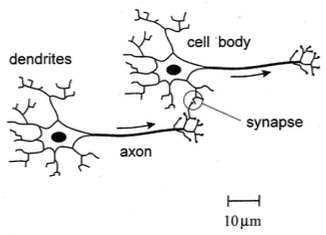
\includegraphics[width = 0.6 \linewidth]{images/biological neuron.png}
    \centering
    \caption{Composizione di due neuroni biologici.}
    \label{biological neuron}
\end{figure}
Da come possiamo notare, esistono vari componenti che costituiscono un 
neurone. In particolare, abbiamo i \emph{dendriti} che rappresentano gli ingressi di un 
neurone mentre le uscite sono rappresentare dagli \emph{assoni}. Su ogni assone viaggia 
un impulso elettrico generato dal neurone stesso quando questo si trova in uno 
stato attivo. Ogni neurone è connesso a migliaia di suoi simili ed ogni 
comunicazione fra questi avviene mediante le sinapsi. Quando l’impulso raggiunge 
proprio le sinapsi, questo provoca il rilascio di sostanze chimiche che attraversano 
la giunzioni ed entrano all’interno di altri neuroni. Ci sono due tipologie di sinapsi, 
eccitatori e inibitori. La prima tipologia permette di aumentare la probabilità che 
un neurone si attivi. Tale probabilità è determinata dal peso associato ad ogni 
sinapsi. Avendo multipli collegamenti, ogni neurone effettua una specie di somma 
pesata degli ingressi che, se maggiore di una determinata soglia, può provocare la 
sua attivazione. 

\section{Reti Neurali Artificiali}
Una rete neurale artificiale è un modello computazionale che, a partire da dei dati 
di input, riesce a produrre un output mediante un meccanismo ispirato a quello 
del cervello umano. Alla base di questa similitudine, tali reti prendono il nome di 
\emph{Artificial Neural Networks (ANN)}. Le prime reti neurali, nate attorno gli anni 
’50, basavano il loro funzionamento sui cosiddetti \emph{percettroni}, neuroni artificiali in 
grado di apprendere e di accumulare esperienza. Ogni rete neurale è composta da 
strati di neuroni, comunemente chiamati \emph{layers}. I dati di input saranno processati 
dai neuroni presenti nell’input layer e da qui, i risultati ottenuti, si propagheranno 
verso i layer nascosti (hidden layers) fino a raggiungere il layer finale di output (Fig. \ref{network structure}).
\begin{figure}[H]
    \centering
    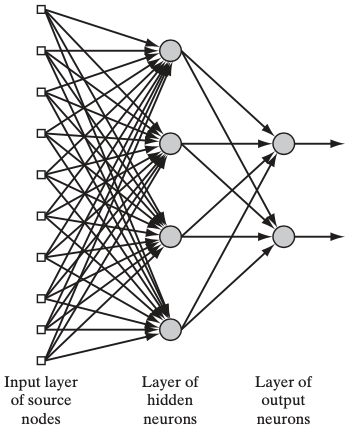
\includegraphics[width = 0.6 \linewidth]{images/netwrok structure.png}
    \centering
    \caption{Struttura di una rete neurale a più livelli.}
    \label{network structure}
\end{figure}
Una componente importante, riguarda la presenza di un insieme di valori 
$w=(w_{k1}, \dots, w_{km})$ chiamati pesi. Ogni peso è rappresentato da un numero reale 
che riflette il grado di importanza di una data connessione, tra due neuroni, in 
una rete neurale \cite{02}. I pesi possono subire dei cambiamenti in base alla tipologia 
di apprendimento della rete. Una buona configurazione dei pesi riduce l’errore di 
predizione e pertanto migliora l’output del modello. Riprendendo il discorso 
dei neuroni, McCulloch e Pitts  \cite{Chakraverty2019} definirono un modello matematico in grado di 
rappresentarli. In particolare, il compito di ogni singolo neurone è rappresentato 
nella figura (\ref{neural neuron}).
\begin{figure}[H]
    \centering
    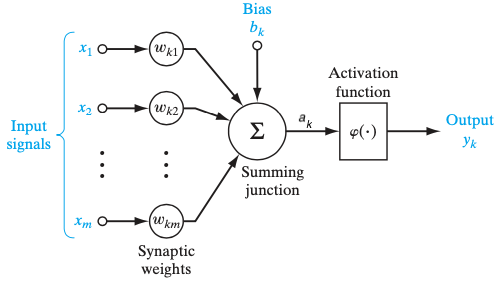
\includegraphics[width = \linewidth]{artificial neuron.png}
    \centering
    \caption{Neurone artificiale.}
    \label{neural neuron}
\end{figure}
Da come possiamo notare, un neurone è una semplice funzione non lineare 
che riceve in input una serie di input $X_{kn}$ e produce in output una variabile $y_k$. 
Il calcolo dell’output, di ogni singolo neurone, è composto da una sommatoria 
degli input, di segno positivo o negativo, moltiplicati prima con i corrispettivi 
pesi e successivamente sommati con una variabile, chiamata bias (pregiudizio), 
che corrisponde alla soglia di attivazione del neurone.
\begin{equation}\label{artificial}
    a_k = \sum_{j=0}^m w_{kj}x_j + b_k 
\end{equation}
Una soglia è utile per determinare se l’informazione in ingresso “$x$” debba essere 
elaborata oppure scartata. Di solito vi è sempre un input $X_0=1$ che renderebbe 
il bias $ b_k $ uguale uguale al primo peso $W_0$, pertanto la formula (\ref{artificial}) può anche 
essere scritta come:
\begin{equation}\label{artificial without bias}
    a_k = \sum_{j=0}^m w_{kj}x_j
\end{equation}
Per poter determinare il valore $y$, dopo aver ottenuto “$a$”, si utilizza una “\emph{funzione 
di attivazione}” non lineare $\varphi(\cdot)$:
\begin{equation}\label{activation function}
    y_k = \varphi(a) = \varphi(\sum_{i=0}^k w_ix_i)
\end{equation}
L’uscita $y$ determinerà l’attivazione del prossimo neurone. Se il valore ricevuto è 
maggiore di zero, allora il neurone si attiverà, altrimenti resterà spento.
\begin{equation}\label{activation function}
    y_k = \left\{
        \begin{array}{rl}
        1 & \mbox{if } a_k \geq 0 \\
        0 & \mbox{if } a_k < 0
        \end{array}
        \right.
\end{equation}
Esistono varie funzioni di attivazione, diverse sono elencate in figura (\ref{activation function}).
\begin{figure}[H]
    \centering
    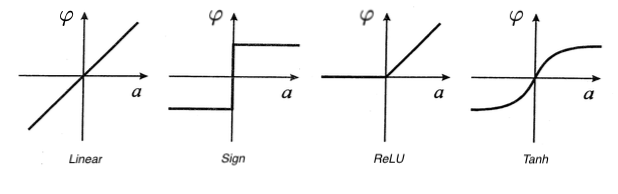
\includegraphics[width = \linewidth]{activation functions.png}
    \centering
    \caption{Varie funzioni di attivazione.}
    \label{activation functions}
\end{figure}
Grazie a questa massiccia interconnessione, le reti neurali artificiali sono in 
grado non solo di imitare il comportamento del cervello umano ma anche di 
svolgere diversi compiti grazie a una opportuna fase di apprendimento. 

\section{Algoritmi di apprendimento}
Lo scambio di dati tra i vari neuroni consente alla rete neurale di poter generalizzare 
anche con dati mai visti nel training set. Questo processo prende il nome di 
“\emph{Apprendimento}”. L’apprendimento di un modello di rete è tipicamente effettuato 
a partire da un insieme di dati di addestramento chiamato training test. All’interno 
di questi insiemi abbiamo la presenza di esempi formati da coppie $(x^j, y^j)$, con 
$j=1,…,n$, dove $y^j$ sta a rappresentare il valore di output desiderato in funzione 
del dato di input $x^j$. Per ricavare il valore target è necessario ricercare gli 
opportuni valori dei pesi, indispensabili a minimizzare l’errore commesso. La 
quantità dell’errore commesso, dal singolo neurone $j$, è esprimibile mediante (\ref{error function}):
\begin{equation}\label{error function}
    \emph{$e_j$}=\hat{y}_j-y_j
\end{equation}
Si può osservare che il calcolo di (\ref{error function}) è riconducibile alla somma dei quadrati 
residua tra il valore stimato $\hat{y}_j$ e quello desiderato $y_j$. L’errore totale derivato da 
tutta la rete è calcolabile prendendo in considerazione la \emph{Funzione di Errore}, a 
volte chiamata anche di \emph{Costo}, esprimibile dal calcolo della seguente formula:
\begin{equation}\label{error function}
    \emph{$E$}=\frac{1}{2}\sum_{j=1}^me_j^2
\end{equation}
dove $m$ rappresenta il numero totale di neuroni presenti nell’output layer.
La funzione di errore $E$ risulta essere molto importate nella fase di apprendimento in quanto misura la distanza 
dalla soluzione ottimale. In generale, la funzione di errore ha diversi minimi (Fig. \ref{minimum and maximum})
\begin{figure}[H]
    \centering
    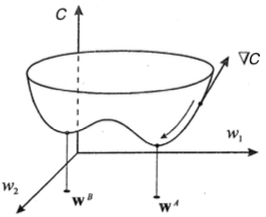
\includegraphics[width = 0.7\linewidth]{cost-function.png}
    \centering
    \caption{Esempio di minimo globale ($w^A$) e locale ($w^B$).}
    \label{minimum and maximum}
\end{figure}
Per ottenere un valore della funzione relativamente basso, l’obiettivo è racchiuso 
nella ricerca del minimo globale. Tale ricerca avviene in maniera iterativa, partendo 
da dei pesi a valori casuali, fino a definirne dei valori fissi. La ricerca dei pesi 
ottimali avviene mediante calcolo delle derivate parziali sulla funzione di errore, 
ovvero del suo vettore gradiente $\nabla{E}$. Questo vettore è utile a definire la direzione 
ed il verso della funzione di errore, in base al set di pesi considerato. Il calcolo delle 
derivate viene svolto dall’algoritmo di \emph{Back Propagation} (discusso nella sezione X 
di questo elaborato). Una rete neurale artificiale può avere vari tipi 
di apprendimento: \emph{Supervisionato, Semi-Supervisionato, Non-Supervisionato} e 
con \emph{Rinforzo}. La scelta di quale usare dipende dalla tipologia della rete e dal suo 
campo di applicazione

\subsection{Apprendimento Supervisionato}
In questa tipologia di apprendimento, l’input fornito alla rete contiene una serie di 
dati etichettati. L’apprendimento supervisionato è solitamente utilizzato sia nel 
conteso della classificazione, dove  si vuole mappare le etichette di input a quelle 
di output, che nel contesto della regressione, dove si mira a mappare l’input a un 
output continuo. La corretta associazione comporta una buona generalizzazione 
da parte del modello. L’apprendimento migliora grazie ad una continua variazione 
dei pesi. Questo tipo di apprendimento è svolto utilizzando una ben nota tecnica 
presente allo stato dell’arte, chiamata \emph{Back-Propagation}. La complessità di questo 
tipo di apprendimento deriva dalla quantità di dati presenti nel training set. 
Affinché la rete riesca a generalizzare al meglio, il training set dev’essere composto 
da un numero di esempi adeguato. La giusta quantità di esempi è utile a prevenire 
spiacevoli situazioni di underfitting o di overfitting della rete.

\subsection{Apprendimento Non-Supervisionato}
Quando una rete neurale è sottoposta ad un simile apprendimento, questa riceve 
in input dei dati privi di etichettatura o non strutturati. Lo scopo della rete, 
o del modello, è quello di estrarne una rappresentazione e creare dei cluster 
rappresentativi. Ci sono delle tecniche a supporto di questa tipologia di apprendimento, 
una fra queste è la riduzione della dimensionalità che è applicata in fase 
di pre-elaborazione delle features avente l’obiettivo di eliminare il rumore dai dati 
quando questi sono presenti in grandi quantità. 

\subsection{Apprendimento Semi-Supervisionato}
Un set di input composto da dati etichettati e non, costituisce un sistema di apprendimento 
semi-supervisionato. Questa tipologia di apprendimento rappresenta 
un sistema che si interpone tra i due precedentemente spiegati. I modelli che fanno 
uso di questo approccio di solito utilizzano una piccola quantità di dati etichettati 
e una grande quantità di dati non etichettati. Tale apprendimento porta alla 
creazione di un modello più flessibile rispetto a quello ottenuto dall’apprendimento 
supervisionato.

\subsection{Apprendimento con Rinforzo}
L’ultimo tipo di apprendimento automatico è chiamato Apprendimento con 
Rinforzo. Il suo scopo è quello di costruire un sistema, comunemente chiamato 
\emph{agente}, che abbia l’obiettivo di migliorare le sue performance interagendo con 
l’ambiente che lo circonda. Il miglioramento dell’intero sistema avviene mediante 
dei feedback chiamati appunto rinforzi. Quest’ultimi non hanno nulla a che fare 
con etichette o valori di verità, ma rappresentano un livello di qualità delle azioni 
intraprese dal sistema. Pertanto, differentemente da un sistema supervisionato, 
non ci sono mappature tra l’input e l’output.

\section{Tipologie di reti neurali}
Esistono diverse tipologie di reti neurali, tra queste abbiamo:
\begin{itemize}
    \item \emph{Reti neurali feed forward (FNN)}
    \item \emph{Reti neurali ricorrenti (RNN)}
    \item \emph{Reti profonde (DNN)}
    \item \emph{Reti convoluzionali (CNN)}
\end{itemize}
Nel seguente elaborato verranno trattate solamente le reti neurali convoluzionali 
ma, prima di introdurle, al fine di capire il loro funzionamento, è necessario 
introdurre prima le reti neurali feed-forward, dette anche reti neurali a catena 
aperta.

\subsection{Reti neurali Feed-Forward}
Per facilitare la comprensione del funzionamento di una comune rete neurale, 
si potrebbe partire dallo studio del comportamento di una feed-forward neural 
network. Questa tipologia di rete può essere vista come una funzione matematica 
non lineare capace di trasformare dei dati di input $x=(x_1, \dots, x_m)$, in dati in 
output $y=(y_{k1}, \dots, y_{kn})$. Quello che accade è quindi una transizione delle variabili 
indipendenti ($X_k$) in variabili dipendenti($Y_k$). Possiamo quindi considerare la rete come una 
funzione nella forma $y = y(x;w)$, dove $y$ sta a rappresentare una funzione di $x$ 
e che a sua volta è parametrizzata da $w$.        
% !TEX encoding = UTF-8
% !TEX TS-program = pdflatex
% !TEX root = ../thesis.tex

%**************************************************************
\chapter{METODOLOGIA}
\label{Capitolo3}
\thispagestyle{empty}

Nel capitolo precedente sono stati spiegati tutti i concetti principali che 
compongono un sistema di visione artificiale\index{visione artificiale}, il quale ha lo scopo principale 
di effettuare la comprensione della scena mediante l'utilizzo di tecniche di 
object detection\index{object detection} e di semantic segmentation\index{semantic segmentation}. Oltre a questi concetti, sono 
state definite anche le comuni tecniche di compressione/ottimizzazione\index{compressione} che 
permettono ad un modello di essere eseguito anche su dispositivi a limitate 
risorse\index{risorsa} computazionali\index{computazionale}, relativamente economico, alla portata di tutti. 
L'obiettivo finale dello studio è basato sull'incremento delle prestazioni di 
un modello tramite l'utilizzo di una delle tecniche di compressione/ottimizzazione\index{compressione} 
citate nel capitolo precedente. Nel seguente capitolo vengono 
riportate tutte le metodologie adottate che hanno portato alla realizzazione 
di un metodo personalizzato avente lo scopo prefissato. Il focus principale 
sarà rivolto verso la tecnica di object detection\index{object detection}. È proprio quest'ultima 
tecnica ad essere stata utilizzata maggiormente in questo elaborato. Le
risorse\index{risorsa} computazionali\index{computazionale} richieste da codesta risultano essere onerose. Essendo 
un sistema autonomo implementato all'interno di una centralina dedicata, 
bisogna aver un chiaro prospetto delle potenzialità richieste da un modello di 
visione artificiale per poter raggiungere l'obiettivo finale. Il dispositivo preso 
in riferimento è costituito da un nota scheda di elaborazione embedded\index{embedded}, che 
prende il nome di Nvidia Jetson Nano\index{NVidia Jetson Nano}. Le potenzialità messe a disposizione 
da questa scheda sono state comparate, in termini di Frames-per-Second\index{frame per second (FPS)} 
(FPS), con quelle messe a disposizione sia dal computer del sottoscritto 
che da Google Colaboratory (Colab). Avendo caratteristiche hardware ben 
differenti l'uno dall'altro, si è pensato di creare una comparazione standard 
composta dallo stesso codice eseguito su tutte e tre le diverse architetture\index{architettura}. 
Dopo aver ottenuto i primi risultati dai modelli pre-addestrati, messi gentilmente 
a disposizione da NVidia, questi hanno costituito le baselines ovvero 
i punti di riferimento da cui partire. Per poter ricavare i benchmarks\index{benchmark}, 
tutti i modelli, pre-addestrati e proposto, saranno sottoposti al percorso di 
elaborazione raffigurato in Figura (\ref{flow_chart}). Per la descrizione dell'inferenza\index{inferenza} e per 
visualizzazione dei risultati (benchmarks\index{benchmark}) ottenuti in ogni test, si rimanda la lettura al prossimo capitolo (\ref{Chapter4}).
\begin{figure}
    \centering
    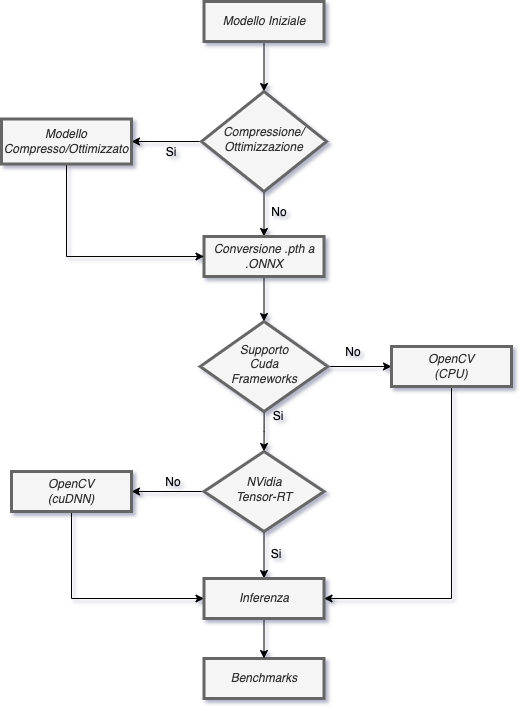
\includegraphics[width = \linewidth]{flow_chart.png}
    \centering
    \caption{Flusso di esecuzione di ogni modello.}
    \label{flow_chart}
\end{figure}

\section{NVidia Jetson Nano}
La Jetson Nano (B01)\index{NVidia Jetson Nano}, presentata nel Marzo del 2019,  è una scheda embedded\index{embedded} 
sviluppata da NVidia che rappresenta il prodotto più piccolo della 
famiglia Jetson. L'utilizzo della scheda è rivolto principalmente verso varie 
applicazioni di intelligenza artificiale, visione artificiale\index{visione artificiale} e robotica. A bordo 
troviamo un processore e una scheda madre che offre una potenza di calcolo 
pari a 128 Cuda cores. L'obiettivo di questa scheda è quello di funzionare 
con reti neurali e offrire le migliori prestazioni quando viene utilizzata per 
eseguire inferenze\index{inferenza}. A differenza di altre architetture\index{architettura}, lo Jetson Nano\index{NVidia Jetson Nano} utilizza 
una precisione Floating point (FP) a 16-bit che lo rende competitivo rispetto 
ad altri device embedded\index{embedded}. Purtroppo non supporta la precisione a 8-bit 
ma è comunque in grado di lavorare con qualsiasi rete disponibile e con 
qualsiasi framework di deep learning\index{deep learning} popolare (es: Pytorch, TensorFlow, 
Keras, Caffe etc.). In questo dispositivo è possibile effettuare sia il rilascio\index{rilascio} 
(deploy) dell'applicazione che l'addestramento della rete ma, in quest'ultimo 
caso, risulta essere lento a causa delle prestazioni computazionali\index{computazionale} ridotte. 
Risulta inoltre possibile effetuare operazioni di transfer learning\index{transfer learning} tra i modelli.
Oltre ad avere il vantaggio delle dimensioni ridotte, un altro principale vantaggio 
della Jetson Nano\index{NVidia Jetson Nano} deriva dall'applicazione dell'acceleratore TensorRT\index{TensorRT}. 
Quest'ultimo esegue un processo di quantizzazione\index{quantization} che è utile a convertire i 
pesi e gli input in precisioni Floating Point inferiori, in modo da preservare 
la memoria che, su una scheda del genere, rappresenta una limitazione. A 
tal proposito, il dispositivo non fornisce alcun tipo di memoria integrata, 
ma esiste la possibilità di aggiungerne una grazie alla presenza di uno slot 
di espansione in cui è possibile alloggiare una scheda micro-sd. Essendo una 
scheda embedded\index{embedded}, a differenza di altri computer che utilizzano alimentatori 
da diversi Watts (W), la Jetson Nano\index{NVidia Jetson Nano} può utilizzare due diversi livelli di 
wattaggio. Il primo, quello da 5W, raggiungibile grazie alla presenza di 
una porta micro-usb, mentre il secondo, quello da 10W, è raggiungibile solo 
grazie all'utilizzo di un alimentatore esterno collegato tramite l'ingresso 
jack. Il massimo livello di performance\index{performance}, raggiungibile dalla GPU, avviene 
proprio tramite l'utilizzo dell'alimentatore esterno. Per rendere l'idea delle 
dimensioni e dell'intera architettura\index{architettura}, in Figura (\ref{jetson}) è riportata la Jetson 
Nano.\index{NVidia Jetson Nano}
\begin{figure}[]
    \begin{minipage}[t]{.45\textwidth}
        \centering
        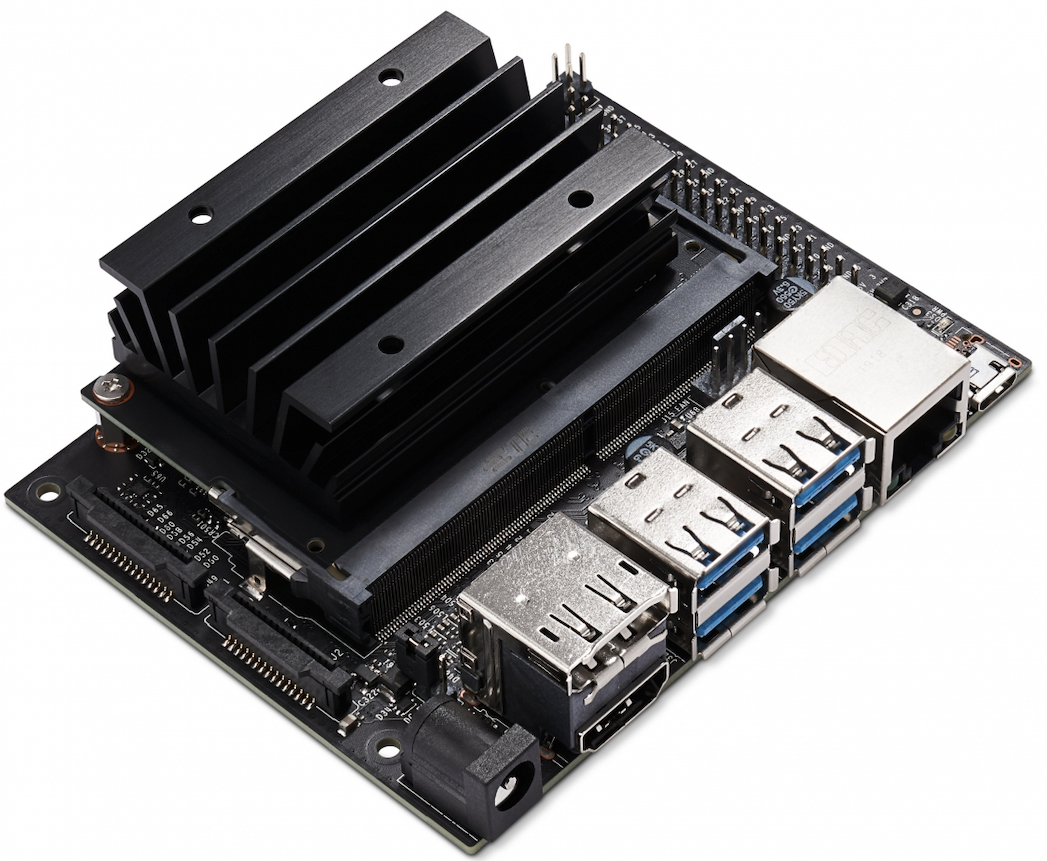
\includegraphics[width=\textwidth]{jetson1.png}
    \end{minipage}
    \hfill
    \begin{minipage}[t]{.45\textwidth}
        \centering
        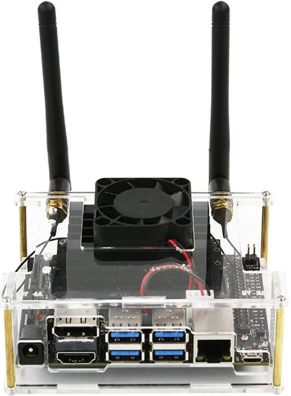
\includegraphics[width= 0.8\textwidth]{jetson2.png}
    \end{minipage}  
    \caption{NVidia Jetson Nano.}
    \label{jetson}
\end{figure}

\section{Modelli}
Il lavoro di tesi è incentrato nello studio di diversi modelli profondi e nell'applicazione, del tutto personalizzata, di una nota tecnica di compressione/ottimizzazione\index{compressione}\index{ottimizzazione} su uno di questi. Lo scopo è quello di aumentare la velocità di inferenza\index{inferenza}, nonché i Frames-Per-Second (FPS)\index{frame per second (FPS)}, in modo da permettere la sua implementazione su diverse architetture\index{architettura} anche con limitate risorse\index{risorsa} computazionali\index{computazionale} (es: Jetson Nano\index{NVidia Jetson Nano}). Per arrivare all'obiettivo finale, si è partito dallo studio delle performance\index{performance} ottenute da diversi modelli pre-addestrati messi a disposizione dalla community di NVidia. Dopo aver ottenuto i risultati, lo studio si è incentrato sull'utilizzo di una particolare architettura\index{architettura} di rete, nota con il nome di \emph{MobileNet-V1}, con l'obiettivo di migliorarla. Successivamente il focus si è spostato nell'implementazione di tale rete in una seconda architettura\index{architettura}, quest'ultima avente il nome di \emph{Single-Shot-Detector (SSD)}. Prima di giungere ai risultati ottenuti, è fondamentale avere un'ampia visione dei modelli utilizzati e di come questi hanno evidenziato le capacità computazionali\index{computazionale} delle architetture\index{architettura} utilizzate. 
\subsection{Modelli pre-addestrati}
I modelli messi a disposizione da NVidia hanno permesso da subito di estrarre le vere potenzialità di tutte le architetture\index{architettura} di studio. Grazie alla presenza di uno script eseguibile nelle librerie jetson utils (ref Jetson utils), sono stati reperiti diversi modelli, allenati su diverse tipologie di datasets\index{dataset}, divisi in due categorie: Object Detection\index{object detection} (Tab. \ref{pre_trained_models_obj_det}) e Semantic Segmentation\index{semantic segmentation} (Tab. \ref{pre_trained_models_sem_seg}).
Tutti i modelli riportati sono stati testati su tutte le architetture\index{architettura} di riferimento. Nuovamente si ricorda al lettore che lo scopo della tesi è aumentare codeste performance\index{performance}. Il produttore ha eseguito alcuni test sulla velocità di inferenza\index{inferenza} solamente su alcuni dei modelli proposti. Per poter visualizzare i risultati ottenuti, si rimanda la lettura al capitolo successivo.
\begin{table}[]
    \renewcommand{\baselinestretch}{1}
    \centering
    \begin{adjustbox}{max width=\textwidth}
    \begin{tabular}{|c||L|L||}
        \hline
        \multirow{2}{*}{\bfseries{MODELLI}} & \multicolumn{2}{c||}{\bfseries{OBJECT DETECTION}}\\            & \bfseries{Dataset} & \bfseries{Risoluzione}\\
        \hline
        \hline
        {\bfseries{SSD-MOBILENET-V1}} & MS COCO & 640$\times$480\\
        \hline
        {\bfseries{SSD-MOBILENET-V2}} & MS COCO & 640$\times$480\\
        \hline 
        {\bfseries{SSD-INCEPTION-V2}} & MS COCO & 640$\times$480\\
        \hline
        {\bfseries{PEDNET}} & MS COCO & 640$\times$480\\
        \hline
        {\bfseries{MULTIPEDNET}} & MS COCO & 640$\times$480\\
        \hline
    \end{tabular}
    \end{adjustbox}
    \vspace{0.5cm}
    \caption{Modelli pre-addestrati utilizzati per l'attività di object detection.}
    \label{pre_trained_models_obj_det}
\end{table}

\begin{table}[]
    \renewcommand{\baselinestretch}{1}
    \centering
    \begin{adjustbox}{max width=\textwidth}
    \begin{tabular}{|c||L|L||}
        \hline
        \multirow{2}{*}{\bfseries{MODELLI}} & \multicolumn{2}{c||}{\bfseries{SEMANTIC SEGMENTATION}}\\            & \bfseries{Dataset} & \bfseries{Risoluzione}\\
        \hline
        \hline
        {\bfseries{FCN-RESNET-18}} & Cityscapes & 512$\times$256\\
        \hline
        {\bfseries{FCN-RESNET-18}} & Cityscapes & 1024$\times$512\\
        \hline 
        {\bfseries{FCN-RESNET-18}} & Cityscapes & 2048$\times$1024\\
        \hline
        {\bfseries{FCN-RESNET-18}} & Pascal Voc & 320$\times$320\\
        \hline
        {\bfseries{FCN-RESNET-18}} & Pascal Voc & 512$\times$320\\
        \hline
    \end{tabular}
    \end{adjustbox}
    \vspace{0.5cm}
    \caption{Modelli pre-addestrati utilizzati per l'attività di semantic segmentation.}
    \label{pre_trained_models_sem_seg}
\end{table}

\subsection{Modello base di riferimento}\label{MBNET}
Per verificare la veridicità dei risultati ottenuti e quelli dichiarati dal produttore, l'intero lavoro di tesi si è concentrato maggiormente nella ricerca e nella costruzione di un modello "from scratch". Per aver un confronto equo, dopo diversi studi focalizzati sulle varie architetture dei modelli pre-addestrati, la scelta è ricaduta sull'implementazione della rete \emph{MobileNet-V1}. Questa decisione è motivata nelle sezioni più avanti quando si discuterà delle tecniche di compressione/ottimizzazione\index{compressione}\index{ottimizzazione} adottate. 
Approfondendo il paper scientifico \cite{howard2017mobilenets}, o scopo degli autori è quello di creare un'architettura di rete dinamica, influenzata dalla presenza di diversi iper-parametri\index{iperparametro}, adattabile in diversi dispositivi compresi quelli mobili. L'architettura\index{architettura} della rete MobileNet-V1 è raffigurata in Figura \ref{mobilenetV1}:
\begin{figure}
    \centering
    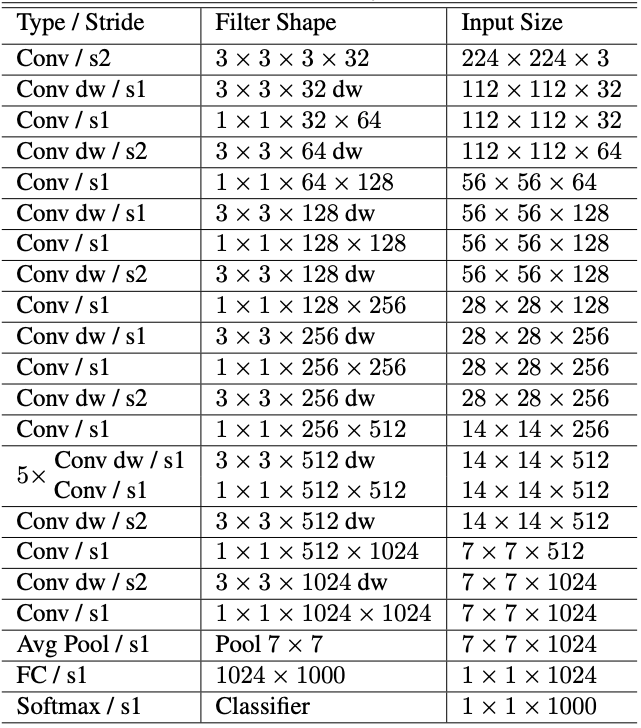
\includegraphics[width = 0.9\linewidth]{mobilenet_architecture.png}
    \centering
    \caption{Architettura MobileNet-V1.}
    \label{mobilenetV1}
\end{figure}
La particolarità che contraddistingue la seguente rete dalle altre è basata sulla presenza di convoluzioni personalizzate chiamate "\emph{Depthwise Separable Convolutions}"  che, a differenza delle comuni convoluzioni, fattorizzano una convoluzione standard prima in una convoluzione profonda e successivamente in una convoluzione 1x1 chiamata "pointwise convolution", formando due layers\index{layer} distinti (Fig. \ref{depth_wise}).
\begin{figure}
    \centering
    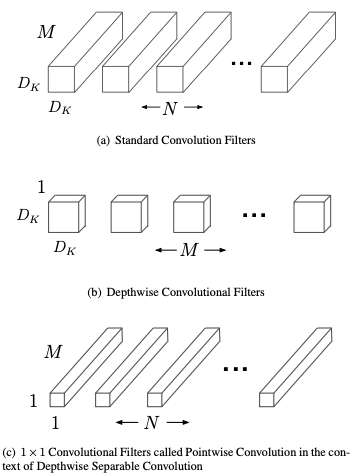
\includegraphics[width = 0.8\linewidth]{depth_wise.png}
    \centering
    \caption{La convoluzione standard (a) viene sostituita da due layers\index{layer}: depthwise convolution (b) e pointwise convolution (c) per costruire un depthwise separable filter.}
    \label{depth_wise}
\end{figure}
La prima convoluzione ha l'obiettivo di applicare un singolo filtro per ogni canale in input, mentre la seconda creare una combinazione lineare dell'output. Lo scopo della fattorizzazione è quello di ridurre drasticamente la computazione e le dimensioni del modello. Tutti i livelli sono seguiti da una normalizzazione batch e una funzione di attivazione\index{funzione di attivazione} ReLU, ad eccezione del livello finale che è un completamente connesso. Il tutto termina con una Softmax utile per la classificazione\index{classificazione}. In totale, MobileNet ha 28 livelli le costituiscono la profondità dell'intera rete. Per costruire una rete a dimensioni ridotte, con un numero di parametri inferiore, beneficiando di un incremento di velocità, gli autori hanno introdotto due tipologie di parametri, uno dei quali risultate molto importanti per raggiungere l'obiettivo di questa tesi. I  due parametri prendono il nome di: 
\begin{enumerate}
    \item \emph{Width Multiplier ($\alpha$)}
    \item \emph{Resolution Multiplier ($p$)}
\end{enumerate}
Il ruolo del width multiplier $\alpha$, un valore tra 0 e 1 compreso, è quello di ridurre le dimensioni della rete in modo uniforme su ogni strato. Per quanto riguarda l'iper-parametro\index{iperparametro} Resolution multiplier $p$,  il suo scopo è quello di accelerare l'inferenza della rete andando ad agire sull'immagine in input e nella rappresentazione interna di ogni livello. In poche parole, l'intento di quest'ultimo parametro\index{parametro} è quello di ridurre la  risoluzione dell'immagine di input, e delle successive sue elaborazioni, per poter incrementare la velocità. Il decremento portato da questo parametro fa sì che la risoluzione possa raggiungere uno dei seguenti valori $p=\{224, 192, 160, 128\}$.
Nel complesso, l'utilizzo di questa architettura\index{architettura} ha permesso la composizione dell'architettura di rete \emph{Single-Shot-Detector (SSD)}. 

\subsection{Modello Single Shot Detector}
Nella sezione precedente sono state riportate tutte le caratteristiche che contraddistinguono una rete MobileNet-V1 rispetto alla concorrenza. Tale rete risulta sostanziale per formare l'ultima architettura\index{architettura} di rete che sarà utilizzata per ricavare i risultati attesi. Il nuovo modello di rete prende il nome di \emph{Single-Shot-Detector (SSD)}.
Una SSD è una rete convoluzionale feed-forward\index{forward} in grado di produrre dei riquadri di delimitazione (bounding-boxes\index{bounding box} o anchor-boxes), di dimensione fissa, con i relativi punteggi associati alle istanze di ogni classe presenti in ognuno dei riquadri. L'ultima operazione applicata, che in gergo viene chiamata "Non-Maximum Suppression" (NMS), è utile per selezionare il riquadro migliore tra tutti quelli prodotti su ogni specifico oggetto. 
L'architettura\index{architettura} una SSD contiene nei primi livelli una "rete base" (backbone\index{backbone}), avente il livello di classificazione finale (FC) rimosso, utilizzata per la classificazione\index{classificazione} delle immagini. Oltre a questa sezione, una SSD si contraddistingue in merito all'aggiunta di ulteriori livelli a seguire, aventi lo scopo di:
\begin{itemize}
    \item \emph{Produrre feature-map multi-scala}\index{feature map}: l'idea è quella di produrre previsioni su identificazioni in più scale. Ogni strato convoluzionale aggiunto produrrà una feature map\index{feature map} sulla quale si potranno identificare\index{identificare} gli oggetti in scale diverse. Le dimensioni di questi livelli diminuiranno all'aumentare della profondità della rete;
    \item \emph{Generare delle predizioni}: grazie all'inserimento degli ulteriori livelli, si ha la possibilità di produrre un set di predizioni sulle identificazioni tramite l'utilizzo di un insieme di filtri. Con l'applicazione di un filtro convoluzionale di dimensioni $3x3xp$, dove p sta ad indicare i canali, su ogni cella, l'intero modello riesce a produrre un punteggio per ogni categoria, con tanto di coordinate correlate alla regione di delimitazione. Ogni filtro produrrà un numero di punteggi pari al numero di classi (background\index{background} compreso). Per esempio, in Conv4\_3 (Fig. \ref{SSD_Arch}), viene applicato un filtro 3x3 utile a mappare 512 canali di input in 25 canali di output. Le coordinate prodotte, verranno confrontate rispetto a determinate anchor-boxes associate a diverse posizioni in ogni feature map\index{feature map};
    \item \emph{Generare dei riquadri di delimitazione}: normalmente vengono associati dei riquadri standard (anchor box) ad ogni feature map\index{feature map} risultante dai livelli convoluzionali aggiunti. Il calcolo di un offset permette di generare delle nuove bounding boxes\index{bounding box} che meglio si adattano all'oggetto nell'immagine. 
\end{itemize}
Invece di utilizzare altri metodi, come la finestra scorrevole (sliding windows), per determinare la posizione di ogni oggetto viene sovrapposta una griglia dove, all'interno di ogni cella, è possibile identificare\index{identificare} la presenza di un oggetto. Se non vi ci fosse alcun oggetto all'interno di una regione, allora tale cella sarà classificata come "background"\index{background} e la posizione verrà ignorata. A volte, all'interno di ogni cella, ci possono essere molteplici oggetti, appartenenti a diverse categorie, in forme diverse. Per poterli rilevare, bisogna introdurre i concetti di "\emph{anchor box}" e di "\emph{receptive field}". 
Un anchor-box è un riquadro, di dimensioni predefinite, responsabile della dimensione e della forma di un oggetto all'interno di una cella che a sua volta può avere più di una anchor-box. Durante l'allenamento di una SSD, viene eseguita una fase di corrispondenza tra il miglior l'anchor-box e il riquadro di delimitazione presente nel ground-truth\index{ground truth} delimitante uno specifico oggetto. Dopo aver trovato l'anchor-box con il più alto grado di sovrapposizione ad un oggetto, si può procedere alla predizione della classe e alla localizzazione\index{localizzazione} della sua posizione. Ogni anchor-box e determinato sia da un valore di aspect-ratio che da un livello di zoom. L'aspect-ratio determina la forma di una anchor-box in base all'oggetto sottostante. Il parametro\index{parametro} zoom invece, è utile per specificare la quantità di ridimensionamento di ogni anchor-box rispetto a ciascuna cella.
In ogni feature map\index{feature map}, per ogni anchor-box verranno calcolati i punteggi di tutte le classi c e 4 offset complessivi relativi alla forma dell'anchor-box nel ground-truth\index{ground truth}, per un numero totale di output pari a:
\begin{equation}
    (c+4)kmn
\end{equation}
dove:
\begin{itemize}
    \item $c$: numero di classi (compresa la classe background\index{background});
    \item $4$: numero di offsets per ogni anchor-box;
    \item $k$: numero di anchor-boxes per ogni posizione;
    \item $m \times n$: dimensione feature map\index{feature map};
    \item $(c+4)k$: numero di filtri applicati ad ogni posizione della feature map\index{feature map}.
\end{itemize}
Prendendo sempre in riferimento la Figura \ref{SSD_Arch}, sulla convoluzione 4\_3 di dimensioni $38x38x512$, viene applicato un filtro, di dimensioni $3x3$.
Successivamente verranno calcolate le 4 anchor-boxes che, in maniera individuale, produrranno un numero di output pari a $(c+4)$. Pertanto, tale livello convoluzionale produrrà un output di $38x38x4x(c+4)$.
In termini di numero di anchor-boxes, saranno prodotti $38x38x4=5776$ riquadri. Proseguendo con il calcolo, il numero totale di riquadri generati è per ogni classe è pari a 8732.
La creazione di multiple predizioni sotto forma di riquadri e di punteggi, è chiamata multibox. 

\begin{figure}
    \centering
    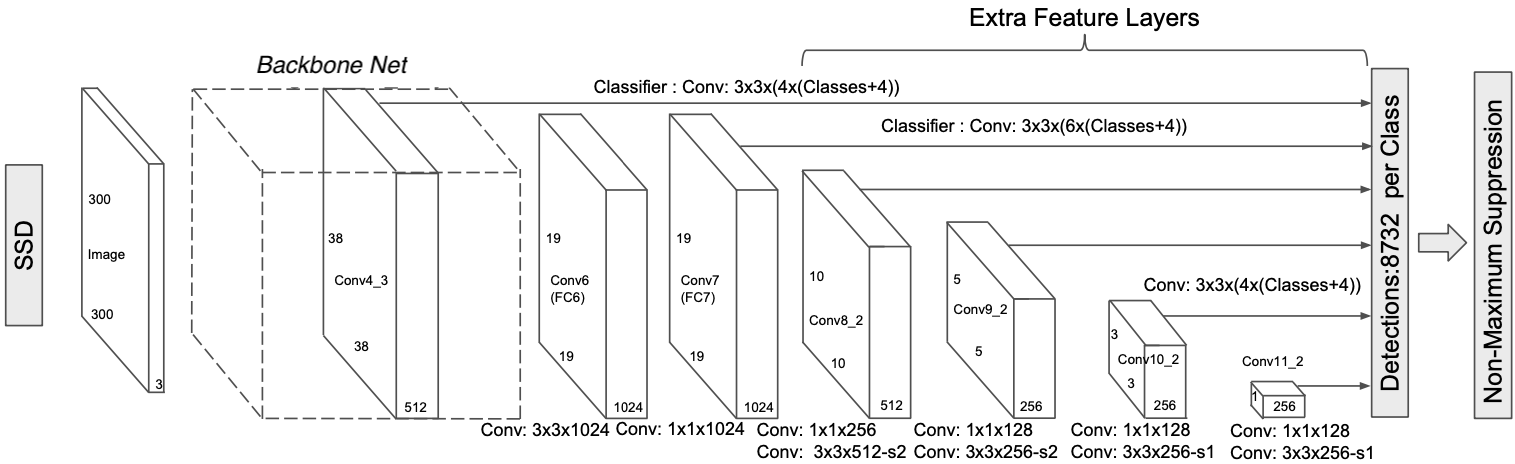
\includegraphics[width =\linewidth]{SSD_architecture.png}
    \centering
    \caption{Architettura Single-Shot-Detector (SSD).}
    \label{SSD_Arch}
\end{figure}

\subsection{Modello Distilled-Single-Shot-Detector (DSSD)}\index{Distilled-Single-Shot-Detector (DSSD)}
Dopo aver elencato, nelle sezioni precedenti, i diversi modelli utilizzati, in questa sezione verrà definito il modello\index{modello} finale proposto su cui si concentreranno tutti gli sforzi del seguente elaborato. Come già accennato, il focus del sottoscritto si è incentrato principalmente verso l'utilizzo di due architetture\index{architettura} di rete utili a compire l'attività di object detection\index{object detection}. Il modello\index{modello} finale si basa nell'implementazione della rete MobileNet-V1 come rete base nell'architettura\index{architettura} Single-Shot-Detector. L'unione tra queste due architetture crea un unico modello nominato \emph{SSD-MobileNet-V1}\index{SSD-MobileNet-V1}.
Il numero di livelli presenti in ogni parte della rete sono:
\begin{itemize}
    \item \emph{27 livelli} (di default sono 28 escludendo l'AvgPool e il Softmax) rappresentanti la rete base (backbone\index{backbone}) da cui è stato rimosso il livello FC;
    \item \emph{8 livelli convoluzionali extra}, seguiti da 8 funzioni di attivazione\index{funzione di attivazione} ReLU.
    \item \emph{6 livelli convoluzionali} utilizzati per la \emph{regressione}\index{regressione};
    \item \emph{6 livelli convoluzionali} utilizzati per la \emph{classificazione}\index{classificazione};
\end{itemize}
Dopo aver inserito la nuova rete base, colleghiamo i livelli depth-wise 12 e 14 alla restante parte della rete SSD. Entrambi i livelli hanno filtri di dimensione pari a $1x1x512x512$ , che a loro volta producono due feature map\index{feature map} aventi profondità 512. L'ultimo collegamento effettuato riguarda l'ultimo livello di convoluzione "pointwise" avente dimensioni $1x1x1024x1024$.
La scelta di questi livelli è attribuita al loro contenuto informativo. In quella determinata posizione, i layers\index{layer} contengono sia feature\index{feature} di alto livello che di basso livello. Dal punto di vista pratico, le predizioni vengono eseguite utilizzando i livelli di classificazione\index{classificazione} e regressione\index{regressione}. Per ogni output prodotto dalla rete base, ci sono differenti livelli collegati (Fig. \ref{SSD_conn}) aventi lo scopo di rilevare gli oggetti aventi diverse dimensioni e proporzioni. Tali livelli sono formati da piccoli kernel\index{kernel} $3x3$ con uno passo (stride\index{stride}) uguale a 1 e funzionano nel seguente modo:
\begin{itemize}
    \item Ogni layer\index{layer} di classificazione\index{classificazione} viene associato ad una particolare anchor-box esistente e all'aspect-ratio di un particolare output della rete. Codesto, durante l'addestramento, impara a rilevare una particolare classe di oggetti;
    \item Ogni layer\index{layer} di regressione\index{regressione} è anch'esso associato a una anchor-box e al suo aspect-ratio. Durante l'allenamento questi apprendono come definire un offset per una determinata anchor-box che è parzialmente contenuta in una anchor-box predefinita. Questa componente pertanto è responsabile di produrre i riquadri di delimitazione.
\end{itemize}
Nelle prossime sezioni verranno elencate tutte le operazioni riguardanti le modifiche apportate a codesta architettura\index{architettura} che hanno permesso di ottenere i risultati sperati.
\begin{figure}
    \centering
    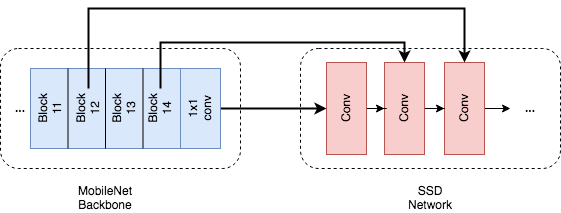
\includegraphics[width =\linewidth]{connection_SSD.png}
    \centering
    \caption{Connessioni tra i livelli della rete base (MobileNet) e i livelli della rete SSD.}
    \label{SSD_conn}
\end{figure}

\section{Compressione/Ottimizzazione del modello proposto}\index{compressione}\index{ottimizzazione}
Avendo definito l'architettura\index{architettura} del modello\index{modello} proposto, nella seguente sezione vengono descritti tutti i suoi impieghi in alcune delle tecniche di compressione/ottimizzazione\index{compressione}\index{ottimizzazione} descritte nel capitolo due. L'affermazione "alcune"sta ad indicare l'esclusione della tecnica di quantizzazione in quanto la minima precisione supportata dalla scheda embedded\index{embedded} Jetson Nano\index{NVidia Jetson Nano} è la FP16 (default). Non potendo applicare la precisione INT8 su quest'ultima, lo studio ha tralasciato l'implementazione pratica di tale tecnica soffermandosi solo a livello teorico. Le altre due tecniche invece, sono state ampiamente utilizzate per condurre dei test sul modello\index{modello} proposto. Di seguito verranno mostrati tutti i procedimenti, eseguiti con entrambe le tecniche, utili a ricavare i risultati finali.

\subsection{Pruning sul modello proposto}\label{pruning_model}
Riprendendo il concetto cardine su cui è focalizzata la tecnica di Pruning\index{Pruning}, è stato possibile svilupparne una sua implementazione con l'aiuto del noto framework di machine learning: PyTorch. Sfortunatamente, la tecnica di pruning\index{Pruning} messa a disposizione da codesto (ancora in fase beta) non migliora i tempi di inferenza\index{inferenza} del modello\index{modello} proposto. Questa causa è da attribuirsi alla non riduzione delle dimensioni dovuta dall'utilizzo di tensori densi all'interno del modello. Un tensore del genere, se riempito di zeri, non esegue calcoli veloci ed inoltre non occupa una dimensione ridotta quando viene memorizzato sul disco. Questa rappresenta una limitazione da parte di questa tipologia di tensori. Di conseguenza, il team di PyTorch afferma che lo scopo, della tecnica messa disposizione, non è incentrato nel garantire incrementi di velocità o risparmi di memoria ma rappresenta un concetto sperimentale. Giusto per non penalizzare solamente PyTorch, anche TensorFlow presenta questa limitazione, ma entrambi hanno intenzione di proseguire lo sviluppo di tale tecnica introducendo nuove migliorie. Attualmente, l'unico fattore da cui si può trarre un vantaggio, riguarda l'applicazione dei programmi di compressione, come per esempio gzip, sui modelli\index{modello} sottoposti al \index{Pruning}. 
Per quanto riguarda il lato implementativo, si è deciso di applicare la tecnica sul modello\index{modello} SSD-MobileNet-V1\index{SSD-MobileNet-V1} precedentemente definito. Come si è potuto notare nel sottoparagrafo apposito, la struttura del modello\index{modello} è composta da diversi livelli quali convoluzionali (Conv2D), Normalizzazione Batch (BatchNorm2D), ReLU (per l'attivazione) e Fully Connected\index{fully connected} (per l'output). Dovendo azzerare i parametri più numerosi, ci si concentrerà maggiormente sui pesi, a loro volta presenti in quantità maggiore nei livelli convoluzionali. 
La tecnica di pruning\index{Pruning} utilizzata è la one-shot.
La funzioni di pruning\index{Pruning} messe a disposizione di PyTorch sono racchiuse nel modulo torch.nn.utils.prune. Grazie alla presenza di un parametro, chiamato "sparsity" (sparsità)\index{sparsità}, si può indicare la percentuale di parametri da azzerare. Le tecniche utilizzate sono le seguenti:
\begin{itemize}
    \item \emph{Unstructured (Non-strutturata)}: reperibile in \emph{torch.nn.prune.l1\_unstructured}. La tecnica applica la potatura in base al magnitudo di ogni peso\index{peso} (norma L1)\index{norma L1}, in maniera individuale in ogni livello. Questa rappresenta la forma più semplice di potatura di un modello;
    \item \emph{Structured (Strutturata)}:  utilizzabile con \emph{torch.nn.prune.ln\_structured}. Questa tecnica incide direttamente sui canali di output andando a rimuovere la porzione di filtri con il punteggio più basso nel livello convoluzionale. La seguente tecnica risulta essere meno fedele rispetto a quella non strutturata;
    \item \emph{Global Unstructured (Globalmente Non-strutturata)}: richiamabile tramite \emph{torch.nn.prune.global\_unstructured}, rappresenta la tecnica che ci fornisce un riscontro globale sulla quantità di pesi da poter rimuovere nell'intero modello\index{modello}.
\end{itemize}
L'API permettono facilmente di utilizzare il modello\index{modello} sia con i parametri originali oppure direttamente con i parametri potati preservando in quest'ultimo caso la struttura originale. Semplicemente, i tensori originali vengono salvati sotto il nome di "\emph{weigth\_orig}", mentre quelli potati vengono salvati in un apposito buffer, chiamato "\emph{weigth\_mask}", contenente tutte le maschere nulle. L'applicazione delle maschere di zeri avviene mediante l'utilizzo di un \emph{forward hook}. Giusto per riportare una breve descrizione, un forward hook è una funzione che viene eseguita quando viene chiamato il metodo "forward"\index{forward} o "backward". Lasciando entrambi i seti di pesi, le dimensioni del modello aumenteranno quando questo verrà salvato su disco. Non essendo lo scopo finale, si procederà ad eliminare i pesi originali rendendo permanenti quelli presenti nella maschera. Per fare ciò è possibile richiamare il metodo \emph{prune.remove}. 
Per quanto riguarda lo spazio occupato in memoria, le tecniche di potatura sembrano avere una relazione lineare con la dimensione di un modello compresso. Questo fenomeno accade a causa della serializzazione effettuata dagli algoritmi di compressione.
Questo benefit è molto richiesto, sia in fase di rilascio\index{rilascio} che di inferenza\index{inferenza}, su un dispositivo con bassa disponibilità su disco. Ovviamente, maggiore sarà l'indice di sparsità\index{sparsità} e maggiore sarà lo spazio recuperato. 

\subsection{Knowledge Distillation sul modello proposto}\index{Knowledge Distillation}\label{KD_steps}
Terminata l'analisi sulle possibili applicazioni della tecnica di Pruning\index{Pruning}, e a quali vantaggi e svantaggi può portare, in questa sezione saranno analizzati tutti gli aspetti derivanti dall'implementazione della seconda tecnica di compressione/ottimizzazione\index{compressione}\index{ottimizzazione}. Il modello finale, derivante dall'applicazione della tecnica di Knowledge distillation\index{Knowledge Distillation}, è stato ricavato tramite l'esecuzione dei sei seguenti passaggi mostrati in Figura \ref{steps_KD}.
\begin{figure}
    \centering
    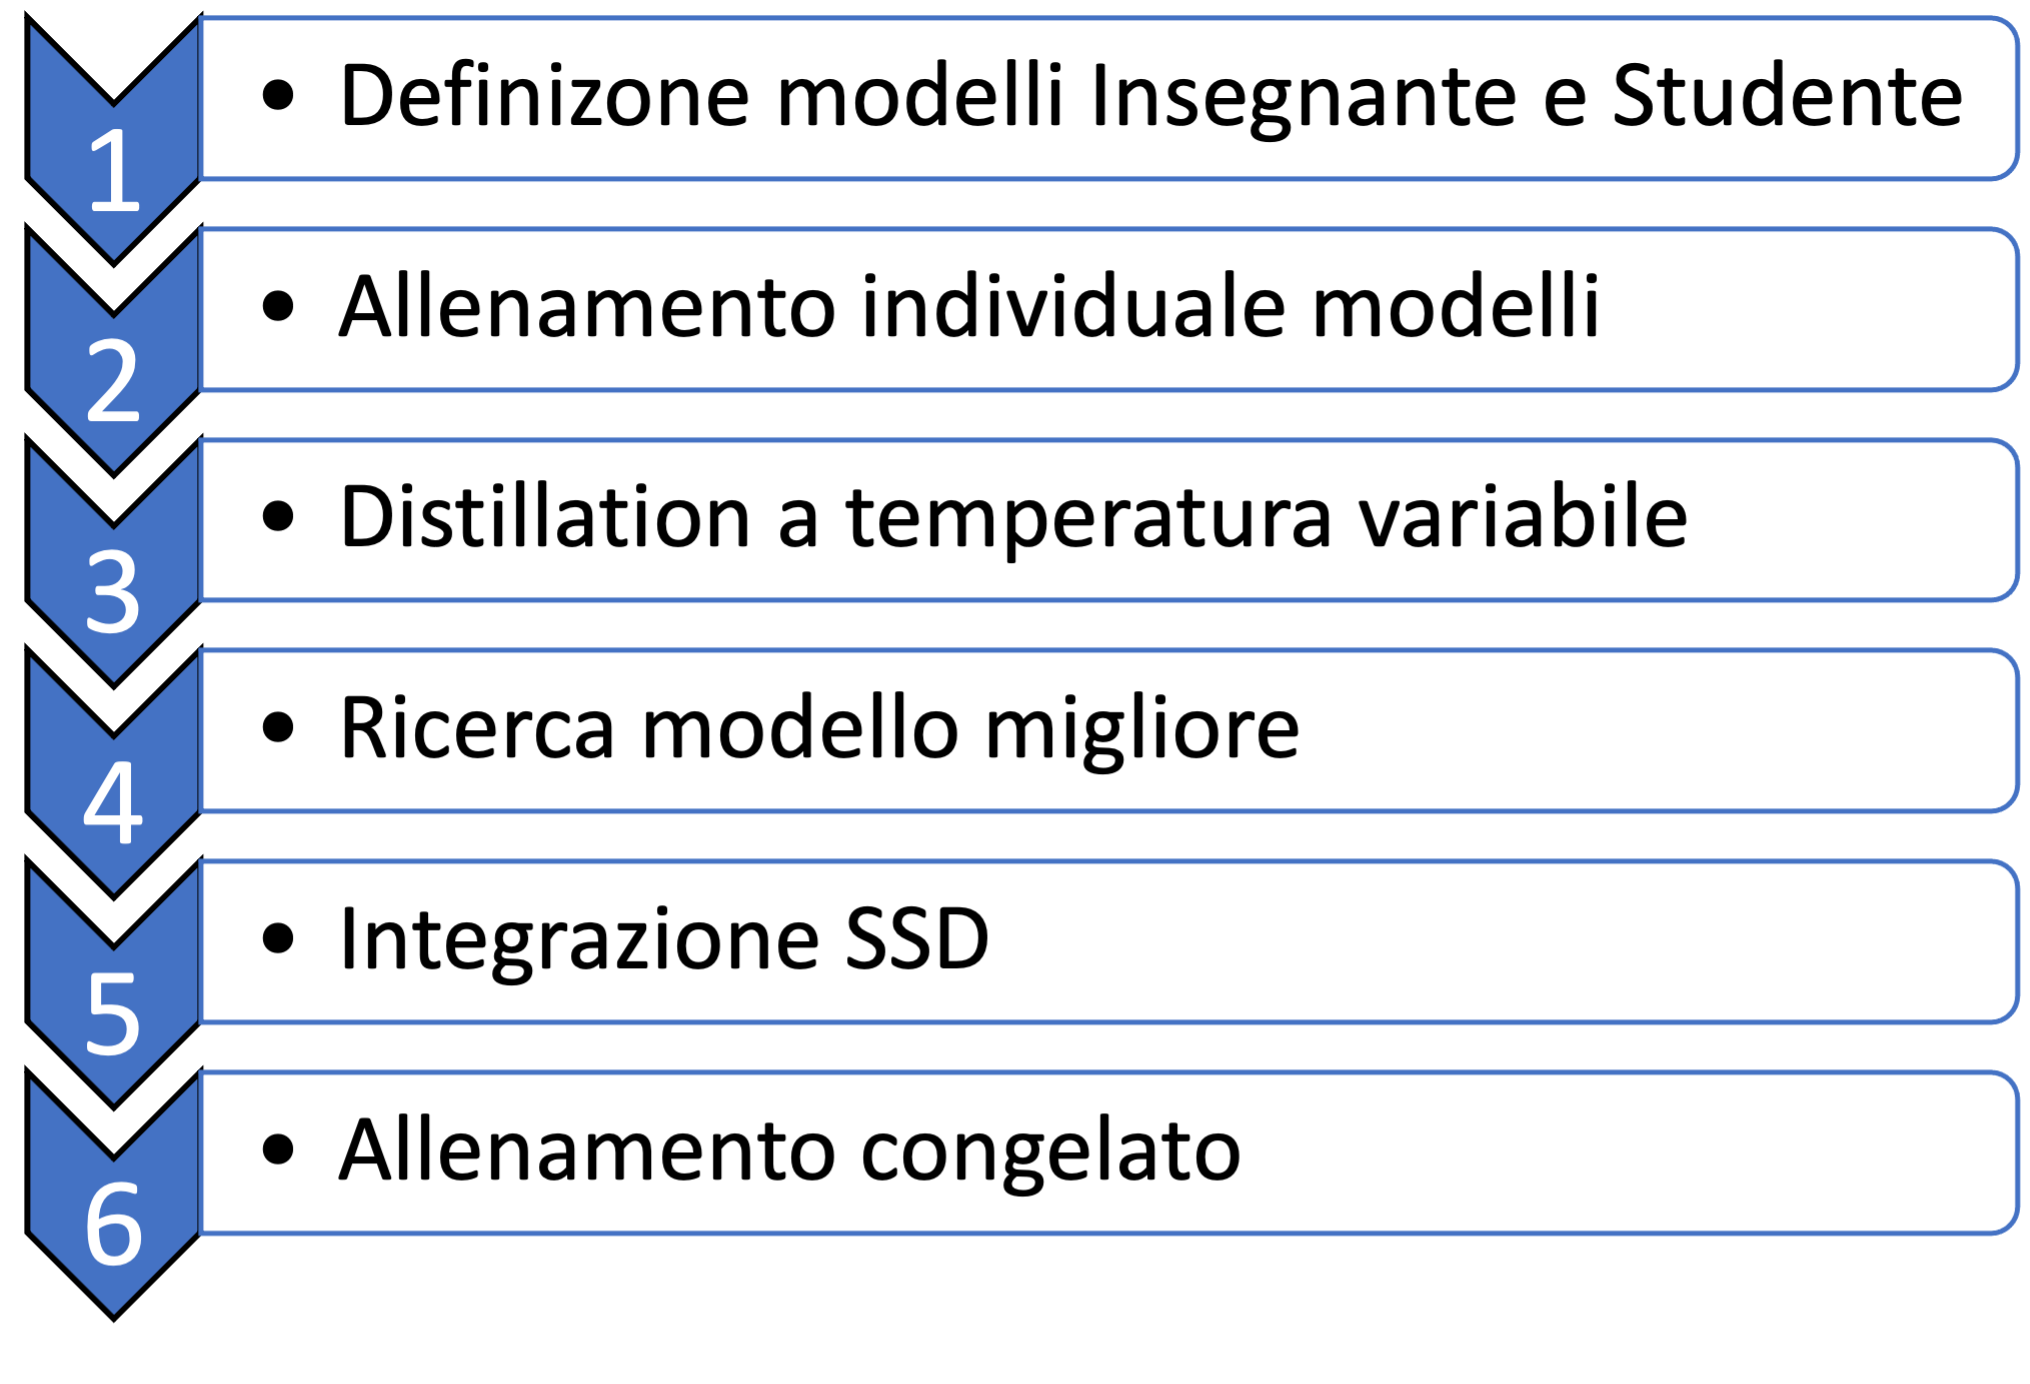
\includegraphics[width =\linewidth]{steps_KD.png}
    \centering
    \caption{Steps per la produzione del modello distillato finale.}
    \label{steps_KD}
\end{figure}

\subsubsection{1. Definzione modelli Insegnante e Studente}
Per la generazione del modello\index{modello} distillato, occorre possedere un modello Insegnante in grado di poter trasmettere la propria conoscenza verso un altro modello. Il modello insegnante utilizzato è il modello base di riferimento (Sezione \ref{MBNET}) MobileNet-V1. Prendendo in riferimento la sua architettura\index{architettura}, affinché possa essere applicato il concetto di Knowledge distillation\index{Knowledge Distillation}, che si basa nel trasferire la conoscenza da un modello di grande dimensioni verso un modello di piccole dimensioni, bisogna creare un secondo modello chiamato Studente. Secondo la letteratura, l'architettura\index{architettura} dello studente dovrà essere simile, in termini di profondità, a quella dell'insegnante. Per soddisfare il seguente vincolo,  ci viene in aiuto l'iper-parametro\index{iperparametro} "width multiplier" ($\alpha$), ideato direttamente dagli autori della rete di riferimento. L'integrazione di tale permette di non incidere sulla profondità della rete ma bensì sul suo numero di parametri, raggiungendo un costo computazionale\index{computazionale} pari a:
\begin{equation}
    D_K \cdot D_K \cdot \alpha M \cdot D_F \cdot D_F + \alpha M \cdot \alpha N \cdot D_F \cdot D_F
\end{equation}
dove:
\begin{itemize}
    \item $D_K$: Dimensioni spaziali del kernel\index{kernel} in una convoluzione;
    \item $D_F$: Dimensioni spaziali feature map\index{feature map};
    \item $M$: numero di canali in input;
    \item $N$: numero di canali in output;
    \item $\alpha$: width multiplier compreso tra 0 e 1 incluso.
\end{itemize}
Il valore del parametro\index{parametro} $\alpha$ utilizzato è pari a 0.25. Moltiplicando tale valore al numero di canali di input e di output, si ottiene un modello più piccolo, di un fattore pari a $1/4$, rispetto al modello insegnante concepito con un valore standard $\alpha=1$. Per facilitare i prossimi calcoli, non è stato ritenuto opportuno implementare anche l'iper-parametro\index{iperparametro} "resolution multiplier" (\emph{p}) in quanto interferente con le diverse dimensioni delle feature map\index{feature map} generate nel comparto SSD. Tralasciando questo elemento, gli autori di MobileNet-V1 affermano che un modello ricavato da tale parametro, oltre ad avere delle dimensioni ridotte e un costo computazionale\index{computazionale} minore, ha un livello di accuratezza\index{accuratezza} leggermente minore rispetto al modello\index{modello} più grande (insegnante). 

\subsubsection{2. Allenamento individuale modelli}
Giunti a questo punto, i modelli a disposizione sono due; un modello Insegnante e un modello Studente. Per poter eseguire gli steps successivi, occorre allenare entrambi i modello\index{modello} per poter ricavare le loro accuratezze\index{accuratezza} utili in seguito. Pertanto, si il seguente step si basa nell'allenare entrambi i modelli sulle immagini fornite dal dataset\index{dataset} "\emph{Open Images}". Le categorie utilizzate, rappresentanti le etichette\index{etichetta} (labels), essendo in un contesto di guida autonoma\index{autonoma}, sono le seguenti: Bicicletta, Bus, Auto, Motociclo, Persona, Semaforo, Cartello stradale e Camion. Ogni modello verrà addestrato per un numero totale di 1000 epoche sull'intero set di allenamento (training set). Il reperimento delle immagini è avvenuto grazie a uno script in grado di creare tre diversi insiemi: allenamento, test e valutazione. In totale, il numero di immagini suddiviso per ogni categoria è riportato nella Tabella \ref{images_train}.
\begin{table}
    \centering
    \begin{adjustbox}{max width=\textwidth}
    \begin{tabular}{|c|c|}
        \hline
        \bfseries{Categorie} & \bfseries{\#Immagini}\\
        \hline
        \hline
        Biciclette & 536 \\
        \hline
        Bus & 157 \\
        \hline
        Auto & 3616 \\
        \hline
        Motocicli & 206\\
        \hline
        Persone & 12094\\
        \hline
        Semafori & 102\\
        \hline
        Segnali stradali & 63\\
        \hline
        Camion & 159\\
        \hline
        \hline
        {\bfseries{Totale}} & {\bfseries{16933}} \\
        \hline
    \end{tabular}
    \end{adjustbox}
    \vspace{0.5cm}
    \caption{Numero di immagini per ogni cateogria.}
    \label{images_train}
\end{table}
La somma del numero delle immagini costituisce un insieme di 16933 elementi, tutti suddivisi nei tre insiemi. Tutti gli allenamenti sono stati eseguiti esclusivamente sull'architettura\index{architettura} Google Colaboratory Pro per una ragione legata prettamente alla velocità temporale messa a disposizione da un hardware costruito ad hoc. Oltre al parametro $\alpha$, gli iper-parametri\index{iperparametro} utilizzati durante l'allenamento riguardano: batch size = 8, learning rate = 0.1, momento = 0.9 e weigth decay = 1e-4. Per quanto riguarda la risoluzione delle immagini in input, queste venivano ridimensionate a una risoluzione pari a 224x224. Per quanto riguarda i tempi di allenamento, sempre su 1000 epoche, il modello insegnante ha impiegato circa 11 ore per concludere contro le 9 ore impiegate dal modello studente. La riduzione dei tempi di allenamento è dovuta alle ridotte dimensioni del modello studente rispetto al modello insegnante. 

\subsubsection{3. Distillation a temperatura variabile}
Fino a questo punto sono stati elencati gli elementi fondamentali su cui creare una base di partenza. Avendo a disposizione i due principali modelli, si procede con la vera e propria applicazione della tecnica di Knowledge distillation\index{Knowledge Distillation}. Prendendo sempre in riferimento tutti i concetti riportati nella sezione \ref{KD_distill} del capitolo 2, l'elemento ritenuto parte integrante di tale tecnica è la temperatura T. Lo scopo è quello avvalersi delle soft-targets\index{soft targets} per realizzare diversi modelli di studenti a diverse temperature, integrando il trasferimento della conoscenza distillata. 
Si ricorda che la nozione di temperatura\index{temperatura} è prettamente legata ad un concetto di generalizzazione\index{generalizzare}. La lista di temperature\index{temperatura} utilizzate è: $T=\{1, 2, 3, 4, 5, 10, 15\}$.
Ogni modello generato deriva anch'esso da un allenamento, ognuno di circa 9 ore, su 1000 epoche, in cui sono stati sottoposti gli stessi insiemi di immagini (batch), sia al modello\index{modello} insegnante che al modello studente base. Il passaggio dell'intero training set ad entrambi i modelli ha permesso di migliorare la perdita generale, che ricordo essere la somma delle perdite dei due modelli. Gli iper-parametri\index{iperparametro}, così come l'intero set di immagini, utilizzati per l'allenamento sono gli stessi utilizzati per allenare i modelli base. Ricapitolando, ciò che si vuole ottenere da questo passaggio riguarda la generazione di multipli modelli di studenti su cui si baseranno i prossimi steps. 

\subsubsection{4. Ricerca modello migliore}
Dopo aver generato i sette nuovi modelli\index{modello} distillati, bisogna chiedersi quale tra questi scegliere. Per ottenere una risposta, bisogna ricavare i tassi di errori (\emph{Errors rates}) sul set di validazione prodotto da ognuno di loro o, in altri termini, bisogna ricavare la curva di apprendimento\index{apprendimento} di ogni modello. Tale curva mette in risalto gli errori effettuati in fase di validazione in ogni epoca. Il valori minimi e massimi sono gli errori presi in considerazione e sono visibili nella Tabella \ref{error_rates_T}.
\begin{table}
    \renewcommand{\baselinestretch}{1}
    \centering
    \begin{adjustbox}{max width=\textwidth}
    {\Large
    \begin{tabular}{|c||L|L||L|L|}
        \hline
        \multirow{2}{*}{\bfseries{MODELLI}} & \multicolumn{2}{c||}{\bfseries{IPER-PARAMETRI}} & \multicolumn{2}{c|}{\bfseries{ERRORI}}\\  & \bfseries{$\alpha$} & \bfseries{T}  & \bfseries{Min} & \bfseries{Max} \\
        \hline
        \hline
        {\bfseries{Insegnante}} & 1 & / & \color{blue}{\bfseries{32}} & \color{blue}{\bfseries{76}}\\
        \hline
        {\bfseries{Studente base}} & 0.25 & / & \color{blue}{\bfseries{40}} & \color{blue}{\bfseries{73}}\\
        \hline 
        {\bfseries{Studente-Dst}} & 0.25 & 1 & \color{red}36 & \color{red}74\\
        \hline
        {\bfseries{Studente-Dst}} & 0.25 & 2 & \color{red}43 & \color{red}76\\
        \hline
        {\bfseries{Studente-Dst}} & 0.25 & 3 & \color{OliveGreen}{\bfseries{38}} & \color{OliveGreen}{\bfseries{76}}\\
        \hline
        {\bfseries{Studente-Dst}} & 0.25 & 4 & \color{red}49 & \color{red}73\\
        \hline
        {\bfseries{Studente-Dst}} & 0.25 & 5 & \color{red}41 & \color{red}73\\
        \hline
        {\bfseries{Studente-Dst}} & 0.25 & 10 & \color{red}50 & \color{red}76\\
        \hline
        {\bfseries{Studente-Dst}} & 0.25 & 15 & \color{red}53 & \color{red}77\\
        \hline
    \end{tabular}
    }
    \end{adjustbox}
    \vspace{0.5cm}
    \caption{Errors Rates dei modelli Insengante, Studente base e Studente distillato (Dst) a diverse temperature\index{temperatura} T. I valori in blu sono quelli di riferimento, mentre quelli verdi rappresentano gli errori derivanti dal modello scelto.}
    \label{error_rates_T}
\end{table}
Per la scelta del modello migliore, affinché venga soddisfatto il principio di generalizzazione, un primo vincolo ci impone di scegliere un modello\index{modello} ricavato da una temperatura\index{temperatura} maggiore di uno. La scelta quindi si restringe ad un range di modelli i cui errori, minimo e massimo, fossero compresi tra gli indici di errore del modello insegnante e del modello studente base. Sempre in riferimento alla Tabella \ref{error_rates_T}, il valore di errore minimo deve essere compreso tra io valori 32 e 40 (incluso), mentre il valore massimo deve essere minore o uguale di 76. Il primo modello che rispetta tali condizioni è quello ricavato da una temperatura\index{temperatura} T=3. Per verificare la giusta scelta del modello, bisogna rimandare la lettura al capitolo successivo dove vengono visualizzate le accuratezze\index{accuratezza} di tutti i modelli e l'andamento della loro curva di apprendimento\index{apprendimento}.

\subsubsection{5. Integrazione SSD}
Preso singolarmente, un modello studente distillato saprebbe solamente effettuare operazioni di image classification senza essere realmente utile in ambito di guida autonoma\index{autonoma} o per attività correlate. Nel seguente elaborato, le spiegazioni sull'architettura\index{architettura} Single-Shot-Detector (SSD) non sono state inserite per pura casualità, ma sono principalmente utili in questo preciso punto di ricerca. L'idea alla base è quella inserire la rete studente come rete base (backbone\index{backbone}) dell'architettura\index{architettura} SSD, costituendo uno degli aspetti centrali del seguente lavoro. In letteratura sono pochi i lavori che hanno affrontato tale tematica, pertanto attualmente rappresenta un punto caldo su cui eseguire ricerca.
Per permettere la fusione tra le due architetture\index{architettura}, bisognava modificare il numero dei canali di input e di output dei restanti livelli convoluzionali costituenti la porzione introdotta dalla rete SSD. Tale modifica ha permesso di far combaciare il numero di canali di output dell'ultimo livello della rete base, con il numero dei canali di input del primo livello convoluzionale introdotto dalla SSD. Oltre ai livelli extra, ovviamente sono stati modificati i medesimi parametri delle convoluzioni utilizzate per il calcolo della regressione\index{regressione} e della classificazione\index{classificazione}. Tutte le modifiche fatte nella seconda parte della rete, sono avvenute utilizzando lo stesso iper-parametro\index{iperparametro} $\alpha$, utilizzato precedentemente per definire il modello studente distillato, quest'ultimo ricoprente ora il ruolo di rete base. 
La nuova rete generata, che il sottoscritto ha deliberatamente intitolato come "{\bfseries{\emph{Disitlled-Single-Shot-Detector (DSSD)\index{Distilled-Single-Shot-Detector (DSSD)}}}}", costituisce l'emblema di tutti gli sforzi fin qui fatti. È proprio con questa rete che si cerca di abbattere le limitazioni computazionali\index{computazionale} presenti sui dispositivi aventi poche risorse\index{risorsa} a disposizione. Nel proseguire la lettura, si scopriranno tutti i benefici introdotti dalla seguente architettura\index{architettura}.

\subsubsection{6. Allenamento congelato}
Di per sé, la nuova rete DSSD\index{Distilled-Single-Shot-Detector (DSSD)} non è ancora in grado di svolgere il proprio task in quanto la seconda componente della struttura, ovvero i layers\index{layer} convoluzionali aggiunti, non sono addestrati. Per preservare l'accuratezza\index{accuratezza} della rete base distillata, segue un allenamento "esclusivo" che tiene in considerazione solo i parametri di quei livelli non ancora addestrati. Questa tecnica in letteratura prende il nome di "\emph{freeze}" (congelare). Grazie al suo utilizzo, i parametri dei livelli sottoposti a tale trattamento, non verranno cambiati durante l'allenamento. Normalmente, quando un modello è sottoposto al training, il suo parametro\index{parametro} "\emph{requires\_grad}" è impostato su \emph{True}. Codesto parametro è utile per fornire un modo semplice adeguato a includere o escludere ogni singolo parametro dalla rete durante la fase di back-propagation\index{back propagation}. Quando questo flag viene impostato come "\emph{requires\_grad=False}", esso va ad escludere il parametro\index{parametro} di riferimento dal ciclo di allenamento. Nello specifico, un simile valore andrebbe ad escludere il calcolo del gradiente\index{gradiente}, di un tensore, durante il passaggio all'indietro (backward). Applicando questo concetto a tutti i parametri di un'intera rete, si sta andando a congelare il suo allenamento. A questo punto ci si chiederebbe quale fosse il senso di addestrare una rete che in realtà non è addestrabile. Ad uno stesso input, una rete congelata risponderà con lo stesso output. Questo comportamento non fa altro che preservare l'accuratezza\index{accuratezza} di un modello e infatti è ciò che si vuol fare con la rete base distillata. Mantenendo la rete base con gli stessi valori, l'obiettivo è quello di allenare la restante parte di rete, ovvero i restanti livelli convoluzionali che seguono il modello distillato. Anche questa volta, l'allenamento è svolto interamente in Google Colaboratory, su un totale di 1000 epoche, con learning-rate=0.01, momentum=0.9 e batch-size=8. Ovviamente il dataset\index{dataset} utilizzato resta sempre Open Images. Finalmente, si può affermare che il modello finale è stato portato a termine e che su questo verranno eseguiti diversi benchmarks\index{benchmark} per ricavare i benefici da esso introdotti.  

\section{Conversione modello}
Tutti i modelli, pre-addestrati e non, fin qui utilizzati, possono essere sottoposti ad inferenza\index{inferenza} solamente previa conversione del loro formato. Quando un modello\index{modello} viene addestrato, specialmente con il framework PyTorch, comunemente viene salvato con estensione ".pth". Grazie a questo formato, è possibile esportare o importare un qualsiasi modello. Tramite l'utilizzo del metodo \emph{torch.save()}, è possibile generare un modello con tale estensione che includesse il proprio \emph{state\_dict()} da importare in un secondo momento con il metodo \emph{load\_state\_dict()}.
Dovendo utilizzare diversi tipi di acceleratori, ampiamente discussi nella prossima sezione, è opportuno trovare un formato comune da poter utilizzare in vari framework.  Il formato selezionato, pienamente utilizzato per lo scambio e per la rappresentazione dei modelli machine learning, prende il nome di \emph{ONNX (Open Neural Network Exchange)}.
Tale formato, del tutto open, definisce un set comune di operatori in grado di garantire interoperabilità tra i diversi framework e un accesso a determinate ottimizzazioni hardware.
La possibilità di conversione è resa disponibile sempre da PyTorch tramite il suo modulo \emph{torch.onnx.export()}.
Oltre a questo, ONNX supporta altri tipi di framework quali TensorFlow, Caffe2, Keras, Microsoft, AWS etc. Dovendo far largo uso dell'acceleratore di inferenza\index{inferenza} come Tensor-RT, o delle librerie OpenCV, sempre discussi nella prossima sezione, possiamo immaginare che una parte dell'elaborazione segua il percorso mostrato in Figura \ref{onnx-converter}.
\begin{figure}
    \centering
    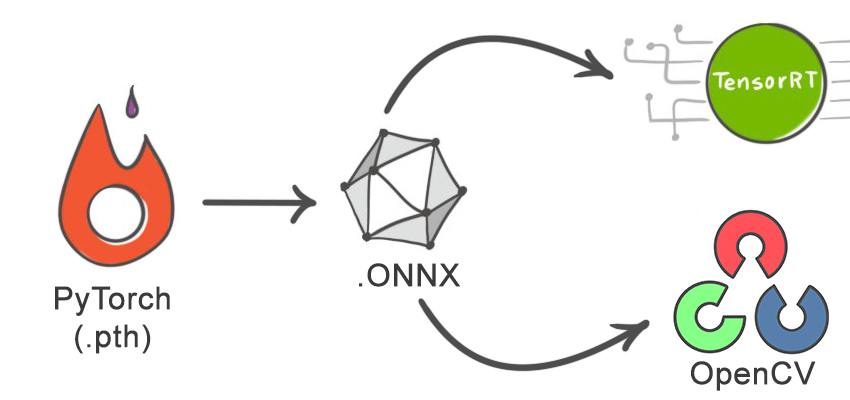
\includegraphics[width = \linewidth]{onnx convert.png}
    \centering
    \caption{Flusso di conversione di ogni modello.}
    \label{onnx-converter}
\end{figure}


\section{Supporto Cuda Frameworks}\label{acceleratori}
\subsection{TensorRT}\index{TensorRT}
\begin{figure}
    \centering
    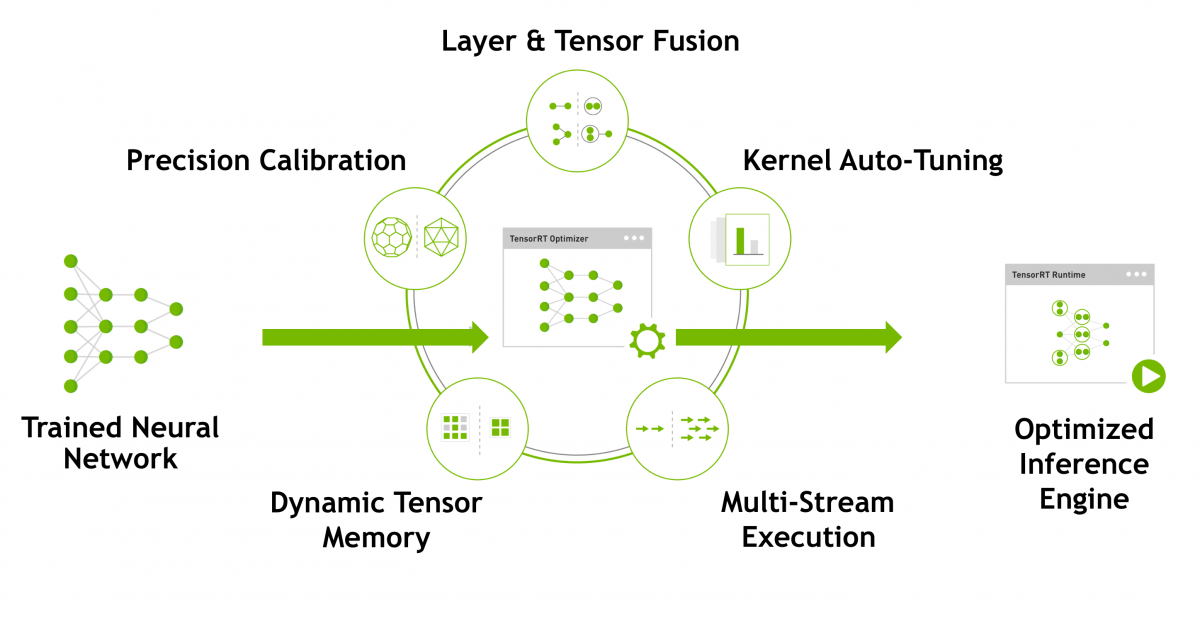
\includegraphics[width = \linewidth]{tensorrtOpt.png}
    \centering
    \caption{Ottimizzazioni si TensorRT sui modelli.}
    \label{tensorrt}
\end{figure}
TensorRT\index{TensorRT} è un framework di machine learning, sviluppato interamente da 
NVidia, che esegue cinque diverse procedure di ottimizzazione\index{ottimizzazione} su architetture 
basate su scheda GPU NVidia (Fig. (\ref{tensorrt})). 
\begin{enumerate}
    \item {\bfseries{\emph{Precision Calibration}}}: in questa ottimizzazione viene eseguita 
    l'operazione di \emph{Quantizzazione}\index{quantization} che permette di mappare tutti i valori 
    dei pesi da una precisione FP32 bit a FP16 bit, creando una perdita 
    di precisione trascurabile.
    \item {\bfseries{\emph{Layer \& Tensor Fusion}}}: la seconda ottimizzazione\index{ottimizzazione} riguarda l'eliminazione 
    di tutti quei layer\index{layer} che non vengono utilizzati, questo è 
    utile per poter evitare calcoli inutili. Successivamente, le operazioni 
    di Convoluzione\index{convoluzione}, ReLU e normalizzazione Batch, vengono fuse in un 
    unico layer (\emph{CBR}). Questa operazione permette di eseguire calcoli 
    in una maniera più veloce ed efficace. Nella Figura (\ref{fusion_tensorrt}) si possono 
    vedere meglio quali sono tutti i layer\index{layer} che vengono fusi da TensorRT\index{TensorRT}.
    \item {\bfseries{\emph{Kernel\index{kernel} Auto-Tuning}}}: la terza ottimizzazione\index{ottimizzazione} viene effettuata direttamente 
    sui filtri utilizzati nella rete. Durante questa fase vengono 
    selezionati i migliori layer\index{layer}, algoritmi e dimensioni di batch in base alla 
    piattaforma GPU di destinazione.
    \item {\bfseries{\emph{Dynamic Tensor Memory}}}: la gestione della memoria viene effettuata 
    proprio in questa ottimizzazione. TensorRT\index{TensorRT} alloca memoria 
    solo per durante il periodo di vita di un tensore scongiurando un 
    sovraccarico di allocazioni permettendo esecuzioni rapide ed efficienti.
    \item {\bfseries{\emph{Multiple Stream Execution}}}: l'ultima ottimizzazione\index{ottimizzazione} riguarda l'elaborazione 
    parallela di multipli flussi di input. Fondamentalmente, 
    questo è possibile utilizzando la libreria CUDA stream.
\end{enumerate}
L'aspetto più importante da ricordarsi, quando si utilizza TensorRT\index{TensorRT}, è che 
bisogna assicurarsi che la procedura di ottimizzazione avvenga sulla stessa 
GPU NVidia che verrà utilizzata per l'inferenza\index{inferenza}. Questo deve avvenire 
in quanto TensorRT\index{TensorRT} utilizza kernel\index{kernel} specifici a seconda della piattaforma 
di destinazione. L'utilizzo di una ottimizzazione\index{ottimizzazione} su una differente scheda 
grafica porta alla creazione di errori in fase di inferenza\index{inferenza}. 
\begin{figure}
    \centering
    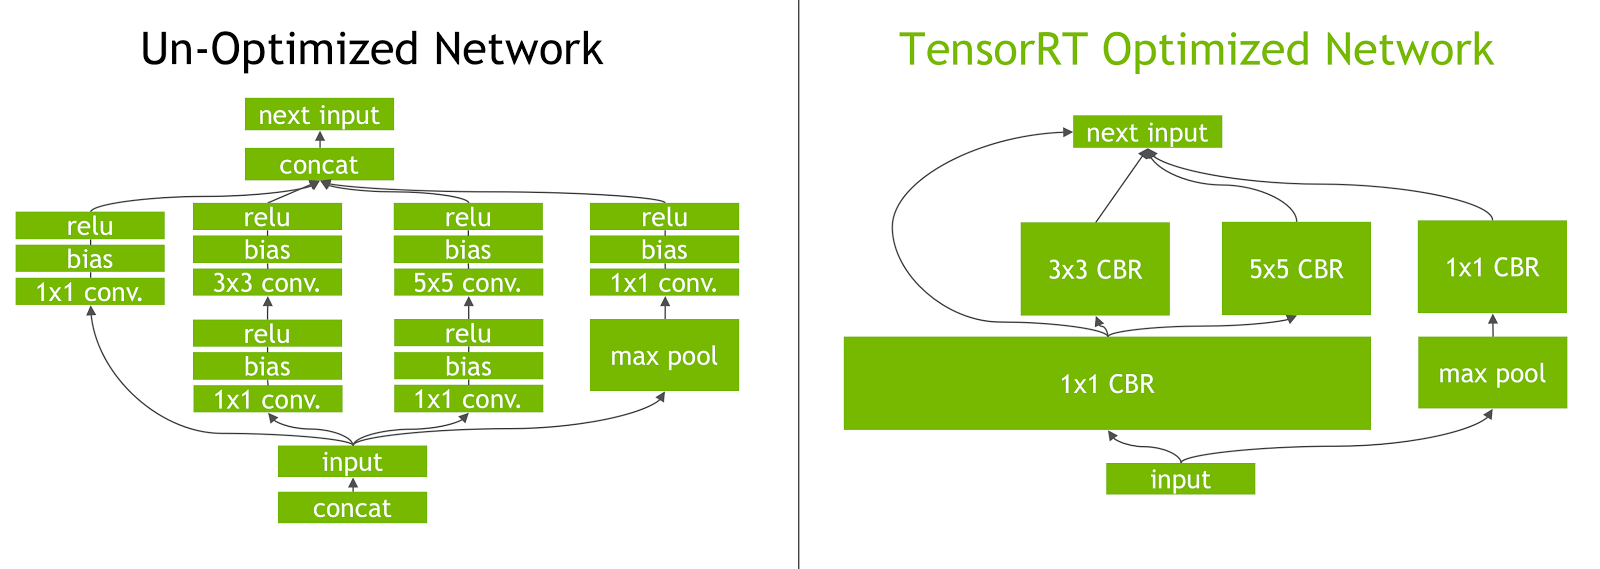
\includegraphics[width = \linewidth]{optTensor.png}
    \centering
    \caption{Fusione dei livelli Convolutional, Batch e ReLU eseguita da TensorRT.}
    \label{fusion_tensorrt}
\end{figure}

\subsection{NVidia Jetson utils}\label{utils}
NVidia dispone di una comunità che supporta l'evoluzione di tutte le sue schede 
embedded\index{embedded}, inclusa la Jetson Nano\index{NVidia Jetson Nano}. Questa associazione ha dato vita 
a delle librerie utilizzate in ambito di computer vision\index{computer vision}, nello specifico rivolto 
alla gestione e alla  progettazione di reti neurali. In ambito di inferenza\index{inferenza}, una 
parte di codeste utilizza l'acceleratore TensorRT\index{TensorRT} per distribuire in modo 
efficiente le reti neurali sulla piattaforma Jetson utilizzata, consentendo 
un miglioramento delle prestazioni e al contempo una migliore efficienza 
energetica. Il codice sorgente messo a disposizione, sviluppato sia in linguaggio 
C++ che in Python (principalmente utilizzato in questo elaborato), 
è composto da diversi scripts che mirano ad eseguire i modelli per svolgere 
svariate attività:
\begin{itemize}
    \item \emph{ImageNet.py}: per attività di Image Recognition;
    \item \emph{DetectNet.py}: per attività di Object detection\index{object detection};
    \item \emph{SegNet.py}: per attività di Semantic Segmentation\index{semantic segmentation};
    \item \emph{PoseNet.py}: per attività di Pose Estimation.
\end{itemize}
Ognuno di questi ha lo scopo di eseguire l'inferenza\index{inferenza} di una apposita rete 
per produrre l'output inerente una specifica attività. In questa tesi sono 
stati utilizzati i primi tre scripts in quanto coerenti con lo scopo prefissato. 
L'input è costituito da uno stream di immagini, video o dati, proveniente 
da una sorgente esterna come per esempio una webcam esterna, collegata 
tramite una porta usb, oppure una webcam collegata tramite interfaccia 
CSI/ISP predisposta direttamente sulla scheda. I frame\index{frame per second (FPS)} di input possono 
provenire da un file avente estensione jpeg, mp4, RTP, RTPS etc. Nel caso 
in cui l'input provenga da una fonte esterna, verrà utilizzato il protocollo 
V4L2 che imposterà il maggior numero di frame rate\index{frame per second (FPS)} alla massima risoluzione 
supportata dalla fonte. Per quanto riguarda l'output, questo può 
essere distribuito nel medesimo formato di input. I codecs supportati dalla 
piattaforma sono i seguenti:
\begin{itemize}
    \item \emph{Decode}: H.264, H.265, VP8, VP9, MPEG-2, MPEG-4 e MJPEG;
    \item \emph{Encode}: H.264, H.265, VP8, VP9 e MJPEG.
\end{itemize}
Le APIs mettono a disposizione anche alcuni scripts che utilizzano il supporto 
CUDA in grado di gestire e manipolare le immagini, che siano di input o 
di output. Ritornando agli scripts principali, ImageNet accetta un'immagine 
in input e restituendone un intervallo di probabilità in output per ogni classe. 
DetectNet, a differenza di ImageNet, oltre a permette di concentrarsi sul rilevamento\index{rilevamento} 
di oggetti, specifica la loro posizione tramite delle bounding boxes\index{bounding box}, 
all'interno del frame in input. Rispetto alla classificazione\index{classificazione} delle immagini, 
le reti utilizzate in questo contesto sono in grado di rilevare multipli oggetti, 
appartenenti alla stessa categoria e non, nell'input specificato. L'output 
prodotto è rappresentato da delle coordinate utili a delimitare i riquadri che 
contraddistinguono ogni singolo oggetto di ogni classe (Fig. \ref{detectnet_result}).
\begin{figure}
    \centering
    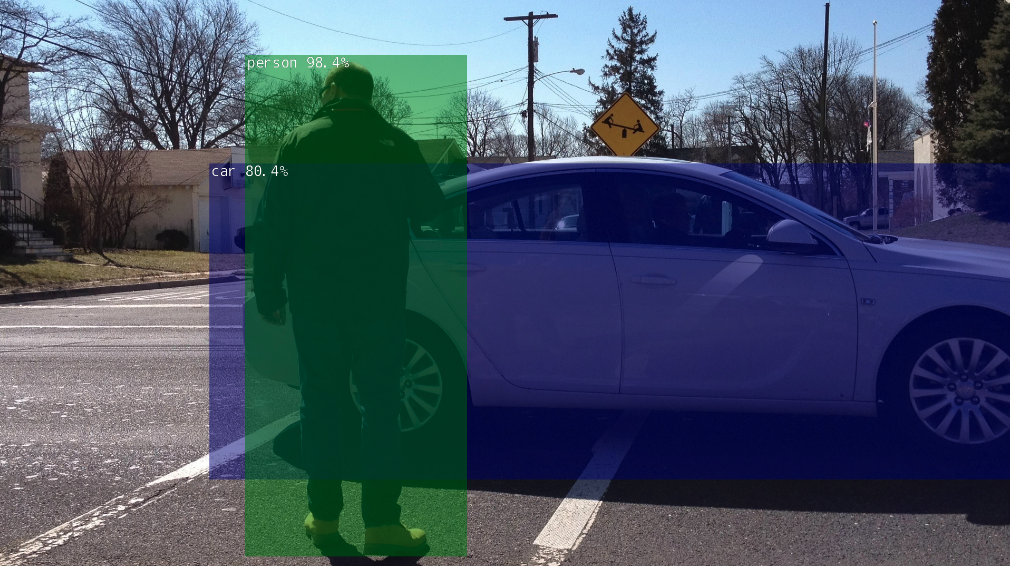
\includegraphics[width = \linewidth]{detectnet_result.png}
    \centering
    \caption{Esempio di ouput prodotto da DetectNet sulla Jetson Nano.}
    \label{detectnet_result}
\end{figure}
Per quanto 
riguarda l'attività di segmentazione semantica\index{semantic segmentation}, questa viene interamente 
svolta dallo script Python Segnet. L'output prodotto da quest'ultimo si 
basa in un'immagine in cui vi è applicata una maschera sovrapposta utile a 
classificare ogni singolo pixel presente nell'immagine di input. Ogni pixel 
della maschera corrisponderà alla classe dell'oggetto sottostante classificato 
(Fig. \ref{segnet_result}).
\begin{figure}
    \centering
    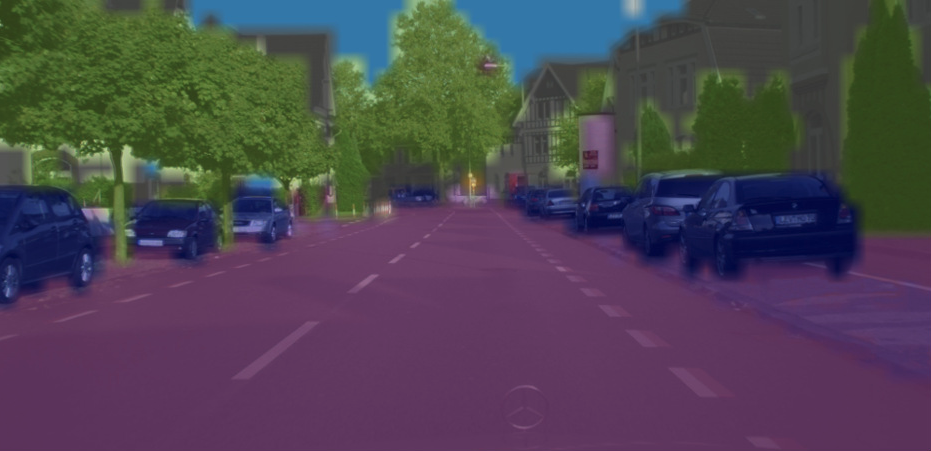
\includegraphics[width = \linewidth]{segnet_result.png}
    \centering
    \caption{Esempio di ouput prodotto da SegNet sulla Jetson Nano.}
    \label{segnet_result}
\end{figure}
Seppur non consigliata come piattaforma su cui effettuare il 
training di un modello, nella repository ufficiale \cite{repo_jetson_nano} viene riportato un link ad 
un'altra repository \cite{repo_pytorch_training} contenente il codice sorgente utile ad addestrare tutti 
i modelli impiegati nelle varie attività. Esiste una documentazione ufficiale 
contenente tutte le informazioni riguardanti gli script citati utilizzabili in 
ogni architettura presente nella famiglia Jetson \cite{Documentation_jetson}. Sia nel training che 
nell'inferenza\index{inferenza} di ogni modello\index{modello}, il framework di ML utilizzato è PyTorch.

\subsection{OpenCV}
Tra le tre architetture utilizzate in questo elaborato, una è sprovvista di una componente fondamentale utile ad accelerare l'allenamento e l'inferenza di un modello. I nuovi macbook pro, nonché il computer del sottoscritto, sono macchine che montano a bordo solo schede grafiche AMD. L'assenza di una scheda grafica NVidia implica l'utilizzo di librerie diverse da TensorRT\index{TensorRT} il quale, a sua volta, fa uso delle librerie CUDA. Quando si verifica una tale limitazione, sia il training che l'inferenza vengono gestiti dalla componente principale di un computer: la CPU. Quando vi è un simile passaggio di elaborazione, le prestazioni computazionali\index{computazionale} sono nettamente inferiori rispetto a quelle ottenute su una scheda grafica. Ed eccoci giunti alla domanda principale: come può essere eseguito un modello su una piattaforma priva di una scheda grafica NVidia? A questo proposito ci viene in aiuto la nota libreria \emph{OpenCV}.
Principalmente utilizzata per lo sviluppo di applicazioni real-time rivolte alla visione artificiale\index{visione artificiale} e all'intelligenza artificiale. É in grado di fornire molteplici funzioni in grado di acquisire, analizzare e manipolare i dati visivi provenienti da uno specifica sorgete di input. Al suo interno, OpenCV possiede un modulo \emph{Deep Neural Network (DNN)} in grado di eseguire l'inferenza di un modello pre-addestrato direttamente su una CPU.
Questa libreria ha permesso di risolvere il problema inerente i test da svolgere sull'architettura Apple a disposizione. A partire dalla versione 4.2.0, OpenCV ha introdotto il pieno supporto alle schede grafiche GPU NVidia, sviluppando un nuovo modulo chiamato "\emph{cuDNN}".
Come ben si intuisce, gli autori hanno permesso di aumentare le performance\index{performance} utilizzando la capacità computazionale\index{computazionale} messa a disposizione di un hardware apposito. Tutto questo ha permesso di creare una sorta di accelerazione, lato inferenza, dei modelli pre-addestrati. Il supporto si è reso interessante per tutte quelle architetture che dispongono di una scheda grafica NVidia, prive di qualunque acceleratore come TensorRT\index{TensorRT}. In questo elaborato, l'architettura che rientra in questa categoria è Google Colaboratory. A causa dell'impossibilità di installazione di TensorRT\index{TensorRT}, si è preferito utilizzare il supporto messo a disposizione da OpenCV per poter ottenere i benchmarks\index{benchmark} voluti. Relativamente facile è risultata l'implementazione di questa funzionalità che ha permesso ad OpenCV di utilizzare la GPU messa a disposizione da Google. Le uniche due righe codice da poter aggiungere alla nostra rete (net) sono le seguenti:
\begin{itemize}
    \item \emph{net.setPreferableBackend(cv2.dnn.DNN\_BACKEND\_CUDA)}
    \item \emph{net.setPreferableTarget(cv2.dnn.DNN\_TARGET\_CUDA)}
\end{itemize}
Il resto del codice è uguale a quello utilizzato per l'inferenza\index{inferenza} su CPU.
Fondamentale risulta la conversione del modello\index{modello} pre-addestrato dal formato \emph{.pth} al formato \emph{.ONNX} per poter essere importato all'interno di OpenCV tramite la funzione \emph{readNetFromONNX()} messa sempre a disposizione nel modulo DNN.
Il supporto fornito da OpenCV ha permesso quindi di ottenere i benchmarks\index{benchmark} su entrambi le architetture utilizzate, ovvero sul macbook pro e su Google Colaboratory.

\section{Frames-per-Second (FPS)}\index{frame per second (FPS)}
La velocità di inferenza\index{inferenza} rappresenta un indicatore di performance\index{performance} di ogni 
modello. Per poterla calcolare, la velocità di inferenza\index{inferenza} è rappresentata dai 
\emph{Frames-per-Second (FPS)} (\ref{FPS_Count}):
\begin{equation}\label{FPS_Count}
    FPS = \frac{1}{Ending \ Time - Starting \ Time}
\end{equation}
Questa misura è variabile e serve per rappresentare tre diversi elementi:
\begin{itemize}
    \item {\bfseries{\emph{Input}}}: ogni rete prende in input una sequenza di frame appartenenti 
    a un video/immagini. Ogni sequenza può avere un numero di FPS variabile. In 
    questo elaborato, vengono testati diversi video a 30FPS e a 60FPS.
    \item {\bfseries{\emph{Netwrok}}}: la velocità che la rete impiega ad effettuare uno specifico 
    task, può essere rappresentata dal numero di FPS. Riconoscere e/o 
    segmentare un oggetto appare essere un'attività onerosa in termini 
    computazionali\index{computazionale}, pertanto una rete è considerata veloce se, oltre a 
    produrre un output adeguato, svolge ogni task in un tempo breve.
    \item {\bfseries{\emph{Output}}}: il risultato prodotto da una rete è visibile solamente a 
    schermo. I video/immagini mostrati/e hanno una velocità di riproduzione 
    che è influenzata dal numero di FPS.
\end{itemize}
Tra le API messe a disposizione da NVidia, citate nella sezione \ref{utils}, 
fondamentale è risultato l'utilizzo dei metodi incaricati di calcolare la 
velocità d'inferenza\index{inferenza}, di input e di output raggiunta da ogni modello\index{modello} su ogni 
attività richiesta.              
% !TEX encoding = UTF-8
% !TEX TS-program = pdflatex
% !TEX root = ../thesis.tex

%**************************************************************
\chapter{RISULTATI SPERIMENTALI}
\label{Capitolo4} \label{Chapter4}
\thispagestyle{empty}
In questo capitolo verranno introdotti i vari dataset di immagini utilizzati per addestrare i modelli. 
Successivamente vengono riportati tutti i risultati sperimentali effettuati 
sui metodi proposti. Le specifiche delle architetture di riferimento, utilizzate per effettuare i vari test, 
sono riportate nella Tabella (\ref{specifiche}).
\begin{table}[htbp]
    \renewcommand{\baselinestretch}{1}
    \centering
    \begin{adjustbox}{max width=\textwidth}
    \begin{tabular}{|c||L|L|L||}
        \hline
        \multirow{2}{*}{\bfseries{ARCHITETTURE}} & \multicolumn{3}{c||}{\bfseries{SPECIFICHE TECNICHE}}\\            & \bfseries{CPU} & \bfseries{GPU} & \bfseries{RAM}\\
        \hline
        \hline
        {\bfseries{JETSON NANO}} & 4 $\times$ ARM Cortex-A57 @ 1.43 GHz & NVidia Maxwell @ 921 MHz & 4 GB 1600 MHz LPDDR4\\
        \hline
        {\bfseries{MACBOOK PRO}} & 8 $\times$ Intel Core i9 @ 2.3 GHz & AMD Radeon Pro 5500M @ 8 GB & 32 GB 2667 MHz DDR4\\
        \hline 
        {\bfseries{COLAB}} & 2 $\times$ Intel(R) Xeon(R) @ 2.20 GHz & NVidia Tesla P-100 @ 16 GB & 26 GB DDR4\\
        \hline
    \end{tabular}
    \end{adjustbox}
    \vspace{0.5cm}
    \caption{Specifiche tecniche delle tre architetture utilizzate.}
    \label{specifiche}
\end{table}

\section{Descrizione dei dataset}
Diversi sono i dataset utilizzati nell'ambito della guida autonoma.
Ogni singolo test viene effettuato utilizzando le immagini contenute nei seguenti dataset: 
\begin{itemize}
    \item {\bfseries{\emph{CityScapes (CS)}}}\cite{Cityscapes}: i dati presenti in questo dataset sono composti da 
    diversi video stereo registrati nelle strade di 50 città diverse. Esistono 
    30 classi diverse raggruppate in otto categorie. Di queste immagini, 
    circa 5000 hanno annotazioni di alta qualità a livello di pixel, mentre altre 
    20.000 hanno annotazioni grossolane. Attualmente, questo dataset 
    rappresenta la pietra miliare della guida autonoma pertanto viene 
    utilizzato in molte ricerche. Nel presente elaborato, precisamente 
    nella sezione dei test di semantic segmentation, vengono utilizzate diverse 
    immagini appartenenti a codesto dataset (Fig. (\ref{cityscapes})), ognuna opportunamente ridimensionata ad una risoluzione diversa.
    \begin{figure}
        \centering
        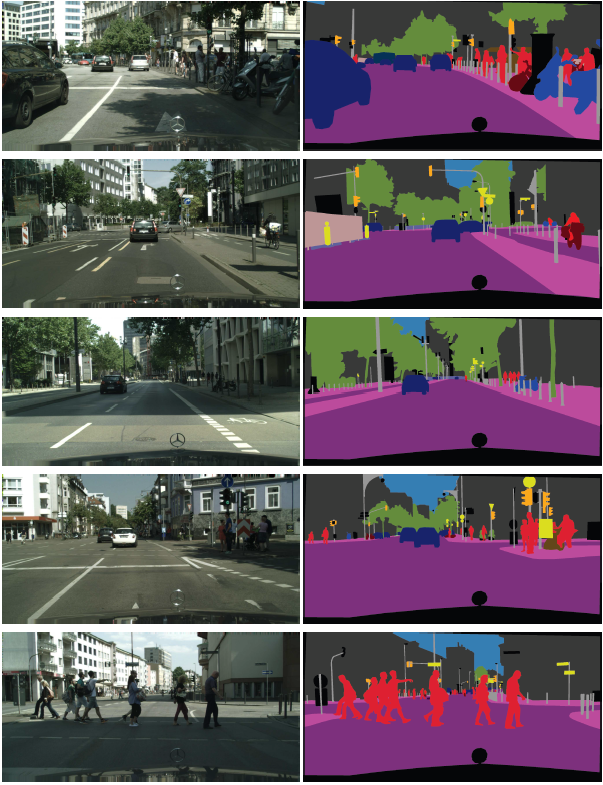
\includegraphics[width = \linewidth]{cityscapes4.png}
        \centering
        \caption{Esempio di immagini presenti in Cityscapes. A destra viene mostrata l'immagine originale mentre a sinistra la sua segmentazione semantica (Ground Truth).}
        \label{cityscapes}
    \end{figure} 
    ($512\times 256$, $1024\times 512$, $2048\times 1024$).
    \item {\bfseries{\emph{PASCAL Visual Object Classes (VOC)}}}\cite{VOC}: il seguente dataset 
    contiene più di 10.000 immagini con all'interno un totale di più di 20.000 
    oggetti raggruppati in 20 classi diverse (Fig. \ref{pascal}). Anche questo dataset, come 
    il precedente, viene utilizzato nella sezione di test per il task di 
    semantic segmentation in questo elaborato. Dettagliatamente, vengono 
    utilizzate delle sue immagini ridimensionate in formato $320\times 320$ e $512\times 320$.
    \begin{figure}
        \centering
        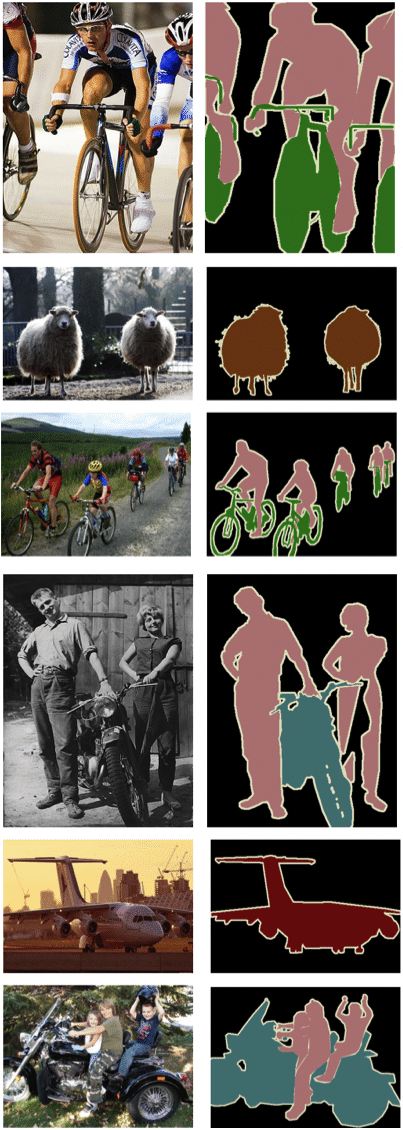
\includegraphics[width = 0.5\linewidth]{PascalVOC.png}
        \centering
        \caption{Esempio di immagini presenti in Pascal VOC. A destra viene mostrata l'immagine originale mentre a sinistra la sua segmentazione semantica (Ground Truth).}
        \label{pascal}
    \end{figure} 
    \item {\bfseries{\emph{MS Common Objects in Context (COCO)}}}\cite{COCO}: realizzato da 
    Microsoft, il dataset contiene più di 300.000 immagini di cui più di 
    200.000 sono etichettate (Fig. (\ref{MSCOCO_dataset})). Gli oggetti presenti sono più di 1.5 milioni e 
    sono raggruppati in 150 classi diverse. Principalmente questo dataset 
    viene utilizzato per attività di object detection, infatti ritorna utile 
    nella sezione di test successiva.
    \begin{figure}
        \centering
        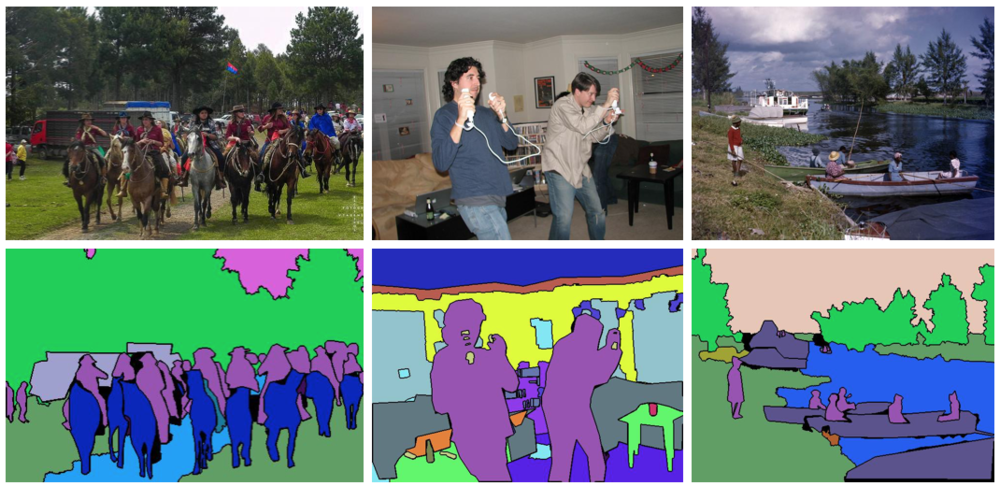
\includegraphics[width = \linewidth]{MSCOCO.png}
        \centering
        \caption{Esempio di immagini presenti in MS COCO. A destra viene mostrata l'immagine originale mentre a sinistra la sua segmentazione semantica (Ground Truth).}
        \label{MSCOCO_dataset}
    \end{figure} 
\end{itemize}

\newpage
\section{Test Performance}
Come brevemente accennato nel capitolo precedente, al fine di capire le 
potenzialità messe a disposizione dalle varie architetture di riferimento, di 
seguito viene riportato un test riguardante la comparazione dei \emph{Frame-per-
Second (FPS)} elaborati da ciascuna macchina. In ogni dataset esistono 
diversi set di immagini, ognuno con diversa risoluzione. Come inferenza, 
si è deciso di sottoporre in input i frame provenienti da sei diversi video 
(.mp4) e da due webcam, tutti aventi diversa risoluzione e numero di FPS (Tab. (\ref{source})).
Nelle tabelle seguenti, contenenti i valori ricavati dai test, sono presenti due tipologie di campi, maggiormente discussi nel capitolo precedente:
\begin{itemize}
    \item {\bfseries{\emph{Out}}}: indica il numero di FPS visualizzabili a schermo;
    \item {\bfseries{\emph{Net}}}: indica il numero di FPS elaborati da una specifica rete durante l'inferenza.
\end{itemize}

\begin{table}
    \renewcommand{\baselinestretch}{1}
    \centering
    \begin{adjustbox}{max width=\textwidth}
    \begin{tabular}{|c||c|c||}
        \hline
        \multirow{2}{*}{\bfseries{Sorgente}} & \multicolumn{2}{c||}{\bfseries{Specifiche Input}}\\            & \bfseries{Qualità} & \bfseries{FPS}\\
        \hline
        \hline
        \RN{1} Video & 240p & 60\\
        \hline
        \RN{2} Video & 360p & 30\\
        \hline 
        \RN{3} Video & 480p & 30\\
        \hline
        \RN{4} Video & 720p &  30\\
        \hline
        \RN{5} Video & 1080p & 30\\
        \hline
        \RN{6} Video & 1080p & 60\\
        \hline
        \RN{7} Webcam1 & 720p & 30\\
        \hline
        \RN{8} Webcam2 & 1080p & 30\\
        \hline
    \end{tabular}
    \end{adjustbox}
    \vspace{0.5cm}
    \caption{Specifiche sorgenti input.}
    \label{source}
\end{table}

\subsection{Test Performance Jetson Nano}
I test effettuati sulla scheda Jetson Nano sono stati eseguiti utilizzando due 
tipologie di librerie diverse, queste sono:
\begin{enumerate}
    \item {\bfseries{\emph{jetson.utils}}};
    \item {\bfseries{\emph{OpenCV}}}.
\end{enumerate}
Le prime sono librerie sviluppate interamente da NVidia che permettono 
l'ottimizzazione di sistemi embedded appartenenti alla famiglia Jetson. 
L'efficienza di questa libreria sta nell'utilizzo dell'SDK \emph{TensorRT} che offre 
una bassa latenza e un throughtput elevato per inferenze deep learning ad 
alte prestazioni. Tutte le applicazioni basate su TensorRT raggiungono 
delle prestazioni fino a 40 volte più veloci rispetto alle piattaforme dotate 
di sola CPU per l'inferenza. Solo le macchine provviste di schede grafiche 
NVidia possono avere questo beneficio in quanto su di esse vi è presente la 
tecnologia \emph{CUDA}, un modello di programmazione parallela che consente 
di ottimizzare l'inferenza grazie a librerie e strumenti di sviluppo basate 
su \emph{CUDA-X} per l'intelligenza artificiale, macchine a guida autonoma, 
elaborazioni ad alte prestazioni e grafica. Ritornando alle jetson.utils, 
queste mettono a disposizione dei modelli utili a compiere svariati compiti, 
come image recognition, object detection, semantic segmentation e pose estimation. 
I test svolti con queste librerie riguardano l'object detection (Tab.(\ref{obj_jetson_utils})) 
e la semantic segmentation (Tab.(\ref{sem_seg_jetson_utils})). A differenza della 
semantic segmentation, i testi per l'object detection vengono fatti su modelli 
pre-addestrati sulle immagine contenute nel dataset MS COCO avente 91 classi di 
elementi differenti. Per un dispositivo embedded di fascia economica, questi test 
raffigurano delle performance promettenti rispetto alla concorrenza.
I test effettuati con OpenCV invece vengono effettuati solo per il compito 
di semantic segmentation in quanto utilizzano file aventi formato \emph{ONNX}, 
messi a disposizione dalla community NVidia, che consentono l'interoperabilità 
tra i diversi framework AI con architetture sottostanti diverse. In poche 
parole, possiamo creare un modello già pre-addestrato e possiamo esportarlo 
in formato .ONNX ed eseguirlo su un'altra macchina con specifiche hardware 
differenti. Le performance ottenute con OpenCV per lo Jetson Nano sono 
visibili nella Tabella (\ref{sem_seg_jetson_utils_opencv_gpu}). Confrontando i 
risultati ottenuti con le jetson.utils, si evince che l'assenza di un 
ottimizzatore porta il sistema ad ottenere delle performance minori. 
Per comprendere le potenzialità offerte da modulo GPU, in Tab. 
(\ref{sem_seg_jetson_utils_opencv_cpu}) vengono riportate le performance 
ottenute dalla sua CPU. Per verificare la veridicità dei test effettuati, 
essendo questi effettuati solamente con le jetson.utils direttamente dal 
produttore della scheda embedded \cite{performance_obj_det_jetson}. Pertanto vengono 
riportati, nelle Tabelle (\ref{average performance jetson utils obj_det}) e (\ref{average performance jetson utils sem_seg}),  
i valori degli FPS medi, sia di Output che della Rete, per entrambe le 
frequenze di FPS in input. Quest'ultime riguardano le performance medie ottenute dall'uso delle jetson.utils, 
mentre quelle visibili nelle Tabelle (\ref{average performance jetson opencv GPU sem_seg}) e (\ref{average performance jetson opencv CPU sem_seg}) rappresentano le performance medie 
ottenute dall'uso delle OpenCV.
\begin{landscape}
    \renewcommand{\baselinestretch}{1}
    \centering
    \begin{table}
        \newarray\First
        \newarray\Second
        \newarray\Third
        \newarray\Fourth
        \newarray\Fifth
        \readarray{First}{16.82&34.48&16.12&33.88&18.6&34.96&18.04&34.05&17.46&33.74&15.6&34.47&11.54&34.78&11.88&34.72}
        \readarray{Second}{15.74&27.31&14.38&27.39&16.24&27.22&15.57&27.07&15.12&26.41&13.93&27&11&27.06&11.09&27.17}
        \readarray{Third}{13.77&21.55&12.38&22&13.93&21.69&13.81&21.67&13.83&21.51&12.31&21.56&9.82&21.81&9.78&21.71}
        \readarray{Fourth}{7.02&8.92&6.83&8.94&6.87&8.93&6.89&8.92&6.91&8.87&6.81&8.89&6.52&8.93&6.6&8.91}
        \readarray{Fifth}{7.02&9.13&6.79&9.12&7.02&9.16&6.96&9.15&6.92&9.07&6.76&9.15&6.57&9.08&6.61&9.08}
        {\scriptsize %
        \begin{tabular}{|c||c|c||c|c||c|c||c|c||c|c||c|c||c|c||c|c||}
            \hline
            & \multicolumn{16}{c||}{ \multirow{3}{*}{\bfseries{\large OBJECT DETECTION (DETECTNET) - JETSON NANO (utils)}}}\\
            & \multicolumn{16}{c||}{}\\
            & \multicolumn{16}{c||}{}\\
            \hline
            \multirow{2}{*}{\bfseries{\large Modelli}} 
            & \multicolumn{2}{c||}{\bfseries{\normalsize Webcam1}} & \multicolumn{2}{c||}{\bfseries{\normalsize Webcam2}} & \multicolumn{2}{c||}{\bfseries{\normalsize \RN{1} Video}} & \multicolumn{2}{c||}{\bfseries{\normalsize \RN{2} Video}} & \multicolumn{2}{c||}{\bfseries{\normalsize \RN{3} Video}} & \multicolumn{2}{c||}{\bfseries{\normalsize \RN{4} Video}} & \multicolumn{2}{c||}{\bfseries{\normalsize \RN{5} Video}} & \multicolumn{2}{c||}{\bfseries{\normalsize \RN{6} Video}}\\            & \bfseries{\footnotesize Out} & \bfseries{\footnotesize Net} & \bfseries{\footnotesize Out} & \bfseries{\footnotesize Net} & \bfseries{\footnotesize Out} & \bfseries{\footnotesize Net} & \bfseries{\footnotesize Out} & \bfseries{\footnotesize Net} & \bfseries{\footnotesize Out} & \bfseries{\footnotesize Net} & \bfseries{\footnotesize Out} & \bfseries{\footnotesize Net} & \bfseries{\footnotesize Out} & \bfseries{\footnotesize Net} & \bfseries{\footnotesize Out} & \bfseries{\footnotesize Net}\\
            \hline
            \multirow{2}{*}{SSD-MOBILENET-V1} & \multirow{2}{*}{\First(1)} & \multirow{2}{*}{\First(2)} & \multirow{2}{*}{\First(3)} & \multirow{2}{*}{\First(4)} & \multirow{2}{*}{\First(5)} & \multirow{2}{*}{\First(6)} & \multirow{2}{*}{\First(7)} & \multirow{2}{*}{\First(8)} & \multirow{2}{*}{\First(9)} & \multirow{2}{*}{\First(10)} & \multirow{2}{*}{\First(11)} & \multirow{2}{*}{\First(12)} & \multirow{2}{*}{\First(13)} & \multirow{2}{*}{\First(14)} & \multirow{2}{*}{\First(15)} & \multirow{2}{*}{\First(16)}\\
            & & & & & & & & & & & & & & & &\\
            \hline
            \multirow{2}{*}{SSD-MOBILENET-V2}& \multirow{2}{*}{\Second(1)} & \multirow{2}{*}{\Second(2)} & \multirow{2}{*}{\Second(3)} & \multirow{2}{*}{\Second(4)} & \multirow{2}{*}{\Second(5)} & \multirow{2}{*}{\Second(6)} & \multirow{2}{*}{\Second(7)} & \multirow{2}{*}{\Second(8)} & \multirow{2}{*}{\Second(9)} & \multirow{2}{*}{\Second(10)} & \multirow{2}{*}{\Second(11)} & \multirow{2}{*}{\Second(12)} & \multirow{2}{*}{\Second(13)} & \multirow{2}{*}{\Second(14)} & \multirow{2}{*}{\Second(15)} & \multirow{2}{*}{\Second(16)}\\
            & & & & & & & & & & & & & & & &\\
            \hline 
            \multirow{2}{*}{SSD-INCEPTION-V2}& \multirow{2}{*}{\Third(1)} & \multirow{2}{*}{\Third(2)} & \multirow{2}{*}{\Third(3)} & \multirow{2}{*}{\Third(4)} & \multirow{2}{*}{\Third(5)} & \multirow{2}{*}{\Third(6)} & \multirow{2}{*}{\Third(7)} & \multirow{2}{*}{\Third(8)} & \multirow{2}{*}{\Third(9)} & \multirow{2}{*}{\Third(10)} & \multirow{2}{*}{\Third(11)} & \multirow{2}{*}{\Third(12)} & \multirow{2}{*}{\Third(13)} & \multirow{2}{*}{\Third(14)} & \multirow{2}{*}{\Third(15)} & \multirow{2}{*}{\Third(16)}\\
            & & & & & & & & & & & & & & & &\\
            \hline
            \multirow{2}{*}{PEDNET}& \multirow{2}{*}{\Fourth(1)} & \multirow{2}{*}{\Fourth(2)} & \multirow{2}{*}{\Fourth(3)} & \multirow{2}{*}{\Fourth(4)} & \multirow{2}{*}{\Fourth(5)} & \multirow{2}{*}{\Fourth(6)} & \multirow{2}{*}{\Fourth(7)} & \multirow{2}{*}{\Fourth(8)} & \multirow{2}{*}{\Fourth(9)} & \multirow{2}{*}{\Fourth(10)} & \multirow{2}{*}{\Fourth(11)} & \multirow{2}{*}{\Fourth(12)} & \multirow{2}{*}{\Fourth(13)} & \multirow{2}{*}{\Fourth(14)} & \multirow{2}{*}{\Fourth(15)} & \multirow{2}{*}{\Fourth(16)}\\
            & & & & & & & & & & & & & & & &\\
            \hline
            \multirow{2}{*}{MULTIPEDNET}& \multirow{2}{*}{\Fifth(1)} & \multirow{2}{*}{\Fifth(2)} & \multirow{2}{*}{\Fifth(3)} & \multirow{2}{*}{\Fifth(4)} & \multirow{2}{*}{\Fifth(5)} & \multirow{2}{*}{\Fifth(6)} & \multirow{2}{*}{\Fifth(7)} & \multirow{2}{*}{\Fifth(8)} & \multirow{2}{*}{\Fifth(9)} & \multirow{2}{*}{\Fifth(10)} & \multirow{2}{*}{\Fifth(11)} & \multirow{2}{*}{\Fifth(12)} & \multirow{2}{*}{\Fifth(13)} & \multirow{2}{*}{\Fifth(14)} & \multirow{2}{*}{\Fifth(15)} & \multirow{2}{*}{\Fifth(16)}\\
            & & & & & & & & & & & & & & & &\\
            \hline
        \end{tabular}
        }%
        \vspace{0.2cm}
        \caption{FPS Performance nell'attività di Object Detection su Jetson Nano (\emph{utils}).}
        \label{obj_jetson_utils}
    \end{table}

    \begin{table}
        \newarray\Firsts
        \newarray\Second
        \newarray\Third
        \newarray\Fourth
        \newarray\Fifth
        \readarray{Firsts}{8.25&48.12&8.37&48.94&20.49&48.92&16.68&48.75&15.7&48.6&9.19&48.24&4.43&48.42&4.63&48.08}
        \readarray{Second}{5.76&12.27&5.57&12.35&8.22&12.34&7.38&12.27&7.46&12.34&5.46&12.3&4.43&12.21&3.96&12.31}
        \readarray{Third}{3.79&3.04&2.56&3.06&4.41&3.06&2.38&3.06&4.31&3.06&2.17&3.06&3.58&3.06&1.79&3.02}
        \readarray{Fourth}{8.96&46.06&7.9&46.44&20.19&46.43&16.37&46.46&15.32&46.63&7.82&46.26&4.78&46.03&4.96&45.98}
        \readarray{Fifth}{8.4&34.31&8.15&34.92&17.15&34.35&13.52&34.26&13.82&34.43&7.42&34.21&4.5&34.61&4.74&34.44}
        {\scriptsize %
        \begin{tabular}{|c||c|c||c|c||c|c||c|c||c|c||c|c||c|c||c|c||}
            \hline
            & \multicolumn{16}{c||}{ \multirow{3}{*}{\bfseries{\large SEMANTIC SEGMENTATION (SEGNET) - JETSON NANO (utils)}}}\\
            & \multicolumn{16}{c||}{}\\
            & \multicolumn{16}{c||}{}\\
            \hline
            \multirow{2}{*}{\bfseries{\large Modelli-Dati}} 
            & \multicolumn{2}{c||}{\bfseries{\normalsize Webcam1}} & \multicolumn{2}{c||}{\bfseries{\normalsize Webcam2}} & \multicolumn{2}{c||}{\bfseries{\normalsize \RN{1} Video}} & \multicolumn{2}{c||}{\bfseries{\normalsize \RN{2} Video}} & \multicolumn{2}{c||}{\bfseries{\normalsize \RN{3} Video}} & \multicolumn{2}{c||}{\bfseries{\normalsize \RN{4} Video}} & \multicolumn{2}{c||}{\bfseries{\normalsize \RN{5} Video}} & \multicolumn{2}{c||}{\bfseries{\normalsize \RN{6} Video}}\\            & \bfseries{\footnotesize Out} & \bfseries{\footnotesize Net} & \bfseries{\footnotesize Out} & \bfseries{\footnotesize Net} & \bfseries{\footnotesize Out} & \bfseries{\footnotesize Net} & \bfseries{\footnotesize Out} & \bfseries{\footnotesize Net} & \bfseries{\footnotesize Out} & \bfseries{\footnotesize Net} & \bfseries{\footnotesize Out} & \bfseries{\footnotesize Net} & \bfseries{\footnotesize Out} & \bfseries{\footnotesize Net} & \bfseries{\footnotesize Out} & \bfseries{\footnotesize Net}\\
            \hline
            \multirow{2}{*}{RN18-CS (512x256)} & \multirow{2}{*}{\Firsts(1)} & \multirow{2}{*}{\Firsts(2)} & \multirow{2}{*}{\Firsts(3)} & \multirow{2}{*}{\Firsts(4)} & \multirow{2}{*}{\Firsts(5)} & \multirow{2}{*}{\Firsts(6)} & \multirow{2}{*}{\Firsts(7)} & \multirow{2}{*}{\Firsts(8)} & \multirow{2}{*}{\Firsts(9)} & \multirow{2}{*}{\Firsts(10)} & \multirow{2}{*}{\Firsts(11)} & \multirow{2}{*}{\Firsts(12)} & \multirow{2}{*}{\Firsts(13)} & \multirow{2}{*}{\Firsts(14)} & \multirow{2}{*}{\Firsts(15)} & \multirow{2}{*}{\Firsts(16)}\\
            & & & & & & & & & & & & & & & &\\
            \hline
            \multirow{2}{*}{RN18-CS (1024x512)}& \multirow{2}{*}{\Second(1)} & \multirow{2}{*}{\Second(2)} & \multirow{2}{*}{\Second(3)} & \multirow{2}{*}{\Second(4)} & \multirow{2}{*}{\Second(5)} & \multirow{2}{*}{\Second(6)} & \multirow{2}{*}{\Second(7)} & \multirow{2}{*}{\Second(8)} & \multirow{2}{*}{\Second(9)} & \multirow{2}{*}{\Second(10)} & \multirow{2}{*}{\Second(11)} & \multirow{2}{*}{\Second(12)} & \multirow{2}{*}{\Second(13)} & \multirow{2}{*}{\Second(14)} & \multirow{2}{*}{\Second(15)} & \multirow{2}{*}{\Second(16)}\\
            & & & & & & & & & & & & & & & &\\
            \hline 
            \multirow{2}{*}{RN18-CS (2048x1024)}& \multirow{2}{*}{\Third(1)} & \multirow{2}{*}{\Third(2)} & \multirow{2}{*}{\Third(3)} & \multirow{2}{*}{\Third(4)} & \multirow{2}{*}{\Third(5)} & \multirow{2}{*}{\Third(6)} & \multirow{2}{*}{\Third(7)} & \multirow{2}{*}{\Third(8)} & \multirow{2}{*}{\Third(9)} & \multirow{2}{*}{\Third(10)} & \multirow{2}{*}{\Third(11)} & \multirow{2}{*}{\Third(12)} & \multirow{2}{*}{\Third(13)} & \multirow{2}{*}{\Third(14)} & \multirow{2}{*}{\Third(15)} & \multirow{2}{*}{\Third(16)}\\
            & & & & & & & & & & & & & & & &\\
            \hline
            \multirow{2}{*}{RN18-VOC (320x320)}& \multirow{2}{*}{\Fourth(1)} & \multirow{2}{*}{\Fourth(2)} & \multirow{2}{*}{\Fourth(3)} & \multirow{2}{*}{\Fourth(4)} & \multirow{2}{*}{\Fourth(5)} & \multirow{2}{*}{\Fourth(6)} & \multirow{2}{*}{\Fourth(7)} & \multirow{2}{*}{\Fourth(8)} & \multirow{2}{*}{\Fourth(9)} & \multirow{2}{*}{\Fourth(10)} & \multirow{2}{*}{\Fourth(11)} & \multirow{2}{*}{\Fourth(12)} & \multirow{2}{*}{\Fourth(13)} & \multirow{2}{*}{\Fourth(14)} & \multirow{2}{*}{\Fourth(15)} & \multirow{2}{*}{\Fourth(16)}\\
            & & & & & & & & & & & & & & & &\\
            \hline
            \multirow{2}{*}{RN18-VOC (512x320)}& \multirow{2}{*}{\Fifth(1)} & \multirow{2}{*}{\Fifth(2)} & \multirow{2}{*}{\Fifth(3)} & \multirow{2}{*}{\Fifth(4)} & \multirow{2}{*}{\Fifth(5)} & \multirow{2}{*}{\Fifth(6)} & \multirow{2}{*}{\Fifth(7)} & \multirow{2}{*}{\Fifth(8)} & \multirow{2}{*}{\Fifth(9)} & \multirow{2}{*}{\Fifth(10)} & \multirow{2}{*}{\Fifth(11)} & \multirow{2}{*}{\Fifth(12)} & \multirow{2}{*}{\Fifth(13)} & \multirow{2}{*}{\Fifth(14)} & \multirow{2}{*}{\Fifth(15)} & \multirow{2}{*}{\Fifth(16)}\\
            & & & & & & & & & & & & & & & &\\
            \hline
        \end{tabular}
        }%
        \vspace{0.2cm}
        \caption{FPS Performance nell'attività di Semantic Segmentation su Jetson Nano (\emph{utils}).}
        \label{sem_seg_jetson_utils}
    \end{table}
\end{landscape}

\begin{landscape}
    \renewcommand{\baselinestretch}{1}
    \centering
    \begin{table}
        \newarray\Firsts
        \newarray\Second
        \newarray\Third
        \newarray\Fourth
        \newarray\Fifth
        \readarray{Firsts}{6.19&18.93&2&19.63&16.41&19.81&14.27&19.69&14.24&19.7&6.62&19.53&4.88&19.24&4.91&19.35}
        \readarray{Second}{3.4&4.99&2&5.53&5.02&5.39&4.75&5.2&4.76&5.2&3.38&4.77&2.86&4.99&2.86&5.36}
        \readarray{Third}{1.09&1.44&1.24&1.45&1.34&1.46&1.34&1.46&1.31&1.46&1.23&1.45&1&1.46&1&1.46}
        \readarray{Fourth}{6.02&17.12&2&17.79&15.41&17.91&13.46&17.76&13.43&17.6&6.56&17.6&4.42&17.33&4.81&17.5}
        \readarray{Fifth}{5.91&14.6&2&14.97&12.9&15.08&11.51&15&11.51&14.98&5.93&14.9&4.51&14.77&4.51&14.85}
        \centering
        {\scriptsize %
        \begin{tabular}{|c||c|c||c|c||c|c||c|c||c|c||c|c||c|c||c|c||}
            \hline
            & \multicolumn{16}{c||}{ \multirow{3}{*}{\bfseries{\large SEMANTIC SEGMENTATION - JETSON NANO (OPENCV - GPU)}}}\\
            & \multicolumn{16}{c||}{}\\
            & \multicolumn{16}{c||}{}\\
            \hline
            \multirow{2}{*}{\bfseries{\large Modelli-Dati}} 
            & \multicolumn{2}{c||}{\bfseries{\normalsize Webcam1}} & \multicolumn{2}{c||}{\bfseries{\normalsize Webcam2}} & \multicolumn{2}{c||}{\bfseries{\normalsize \RN{1} Video}} & \multicolumn{2}{c||}{\bfseries{\normalsize \RN{2} Video}} & \multicolumn{2}{c||}{\bfseries{\normalsize \RN{3} Video}} & \multicolumn{2}{c||}{\bfseries{\normalsize \RN{4} Video}} & \multicolumn{2}{c||}{\bfseries{\normalsize \RN{5} Video}} & \multicolumn{2}{c||}{\bfseries{\normalsize \RN{6} Video}}\\            & \bfseries{\footnotesize Out} & \bfseries{\footnotesize Net} & \bfseries{\footnotesize Out} & \bfseries{\footnotesize Net} & \bfseries{\footnotesize Out} & \bfseries{\footnotesize Net} & \bfseries{\footnotesize Out} & \bfseries{\footnotesize Net} & \bfseries{\footnotesize Out} & \bfseries{\footnotesize Net} & \bfseries{\footnotesize Out} & \bfseries{\footnotesize Net} & \bfseries{\footnotesize Out} & \bfseries{\footnotesize Net} & \bfseries{\footnotesize Out} & \bfseries{\footnotesize Net}\\
            \hline
            \multirow{2}{*}{RN18-CS (512x256)} & \multirow{2}{*}{\Firsts(1)} & \multirow{2}{*}{\Firsts(2)} & \multirow{2}{*}{\Firsts(3)} & \multirow{2}{*}{\Firsts(4)} & \multirow{2}{*}{\Firsts(5)} & \multirow{2}{*}{\Firsts(6)} & \multirow{2}{*}{\Firsts(7)} & \multirow{2}{*}{\Firsts(8)} & \multirow{2}{*}{\Firsts(9)} & \multirow{2}{*}{\Firsts(10)} & \multirow{2}{*}{\Firsts(11)} & \multirow{2}{*}{\Firsts(12)} & \multirow{2}{*}{\Firsts(13)} & \multirow{2}{*}{\Firsts(14)} & \multirow{2}{*}{\Firsts(15)} & \multirow{2}{*}{\Firsts(16)}\\
            & & & & & & & & & & & & & & & &\\
            \hline
            \multirow{2}{*}{RN18-CS (1024x512)}& \multirow{2}{*}{\Second(1)} & \multirow{2}{*}{\Second(2)} & \multirow{2}{*}{\Second(3)} & \multirow{2}{*}{\Second(4)} & \multirow{2}{*}{\Second(5)} & \multirow{2}{*}{\Second(6)} & \multirow{2}{*}{\Second(7)} & \multirow{2}{*}{\Second(8)} & \multirow{2}{*}{\Second(9)} & \multirow{2}{*}{\Second(10)} & \multirow{2}{*}{\Second(11)} & \multirow{2}{*}{\Second(12)} & \multirow{2}{*}{\Second(13)} & \multirow{2}{*}{\Second(14)} & \multirow{2}{*}{\Second(15)} & \multirow{2}{*}{\Second(16)}\\
            & & & & & & & & & & & & & & & &\\
            \hline 
            \multirow{2}{*}{RN18-CS (2048x1024)}& \multirow{2}{*}{\Third(1)} & \multirow{2}{*}{\Third(2)} & \multirow{2}{*}{\Third(3)} & \multirow{2}{*}{\Third(4)} & \multirow{2}{*}{\Third(5)} & \multirow{2}{*}{\Third(6)} & \multirow{2}{*}{\Third(7)} & \multirow{2}{*}{\Third(8)} & \multirow{2}{*}{\Third(9)} & \multirow{2}{*}{\Third(10)} & \multirow{2}{*}{\Third(11)} & \multirow{2}{*}{\Third(12)} & \multirow{2}{*}{\Third(13)} & \multirow{2}{*}{\Third(14)} & \multirow{2}{*}{\Third(15)} & \multirow{2}{*}{\Third(16)}\\
            & & & & & & & & & & & & & & & &\\
            \hline
            \multirow{2}{*}{RN18-VOC (320x320)}& \multirow{2}{*}{\Fourth(1)} & \multirow{2}{*}{\Fourth(2)} & \multirow{2}{*}{\Fourth(3)} & \multirow{2}{*}{\Fourth(4)} & \multirow{2}{*}{\Fourth(5)} & \multirow{2}{*}{\Fourth(6)} & \multirow{2}{*}{\Fourth(7)} & \multirow{2}{*}{\Fourth(8)} & \multirow{2}{*}{\Fourth(9)} & \multirow{2}{*}{\Fourth(10)} & \multirow{2}{*}{\Fourth(11)} & \multirow{2}{*}{\Fourth(12)} & \multirow{2}{*}{\Fourth(13)} & \multirow{2}{*}{\Fourth(14)} & \multirow{2}{*}{\Fourth(15)} & \multirow{2}{*}{\Fourth(16)}\\
            & & & & & & & & & & & & & & & &\\
            \hline
            \multirow{2}{*}{RN18-VOC (512x320)}& \multirow{2}{*}{\Fifth(1)} & \multirow{2}{*}{\Fifth(2)} & \multirow{2}{*}{\Fifth(3)} & \multirow{2}{*}{\Fifth(4)} & \multirow{2}{*}{\Fifth(5)} & \multirow{2}{*}{\Fifth(6)} & \multirow{2}{*}{\Fifth(7)} & \multirow{2}{*}{\Fifth(8)} & \multirow{2}{*}{\Fifth(9)} & \multirow{2}{*}{\Fifth(10)} & \multirow{2}{*}{\Fifth(11)} & \multirow{2}{*}{\Fifth(12)} & \multirow{2}{*}{\Fifth(13)} & \multirow{2}{*}{\Fifth(14)} & \multirow{2}{*}{\Fifth(15)} & \multirow{2}{*}{\Fifth(16)}\\
            & & & & & & & & & & & & & & & &\\
            \hline
        \end{tabular}
        }%
        \vspace{0.2cm}
        \caption{FPS performance nell'attività di Semantic Segmentation su Jetson Nano (\emph{OpenCV - GPU})}
        \label{sem_seg_jetson_utils_opencv_gpu}
    \end{table}

    \begin{table}
        \newarray\Firsts
        \newarray\Second
        \newarray\Third
        \newarray\Fourth
        \newarray\Fifth
        \readarray{Firsts}{1.31&1.48&1.33&1.47&1.68&1.68&1.69&1.74&1.66&1.71&1.51&1.7&1.3&1.59&1.3&1.59}
        \readarray{Second}{0.35&36&0.35&0.36&0.4&0.4&0.41&0.41&0.4&0.4&0.39&0.41&0.37&0.39&0.38&0.4}
        \readarray{Third}{0.09&0.069&0.08&0.08&0.09&0.09&0.1&0.1&0.1&0.1&0.1&0.1&0.09&0.1&0.09&0.1}
        \readarray{Fourth}{1.63&1.88&1.71&1.92&2.18&2.2&2.15&2.22&2.14&2.22&1.88&2.15&1.6&2.06&1.6&2.08}
        \readarray{Fifth}{1.1&1.22&1.11&1.21&1.39&1.39&1.38&1.42&1.37&1.4&1.26&1.38&1.12&1.33&1.12&1.33}
        \centering
        {\scriptsize %
        \begin{tabular}{|c||c|c||c|c||c|c||c|c||c|c||c|c||c|c||c|c||}
            \hline
            & \multicolumn{16}{c||}{ \multirow{3}{*}{\bfseries{\large SEMANTIC SEGMENTATION - JETSON NANO (OPENCV - CPU)}}}\\
            & \multicolumn{16}{c||}{}\\
            & \multicolumn{16}{c||}{}\\
            \hline
            \multirow{2}{*}{\bfseries{\large Modelli-Dati}} 
            & \multicolumn{2}{c||}{\bfseries{\normalsize Webcam1}} & \multicolumn{2}{c||}{\bfseries{\normalsize Webcam2}} & \multicolumn{2}{c||}{\bfseries{\normalsize \RN{1} Video}} & \multicolumn{2}{c||}{\bfseries{\normalsize \RN{2} Video}} & \multicolumn{2}{c||}{\bfseries{\normalsize \RN{3} Video}} & \multicolumn{2}{c||}{\bfseries{\normalsize \RN{4} Video}} & \multicolumn{2}{c||}{\bfseries{\normalsize \RN{5} Video}} & \multicolumn{2}{c||}{\bfseries{\normalsize \RN{6} Video}}\\            & \bfseries{\footnotesize Out} & \bfseries{\footnotesize Net} & \bfseries{\footnotesize Out} & \bfseries{\footnotesize Net} & \bfseries{\footnotesize Out} & \bfseries{\footnotesize Net} & \bfseries{\footnotesize Out} & \bfseries{\footnotesize Net} & \bfseries{\footnotesize Out} & \bfseries{\footnotesize Net} & \bfseries{\footnotesize Out} & \bfseries{\footnotesize Net} & \bfseries{\footnotesize Out} & \bfseries{\footnotesize Net} & \bfseries{\footnotesize Out} & \bfseries{\footnotesize Net}\\
            \hline
            \multirow{2}{*}{RN18-CS (512x256)} & \multirow{2}{*}{\Firsts(1)} & \multirow{2}{*}{\Firsts(2)} & \multirow{2}{*}{\Firsts(3)} & \multirow{2}{*}{\Firsts(4)} & \multirow{2}{*}{\Firsts(5)} & \multirow{2}{*}{\Firsts(6)} & \multirow{2}{*}{\Firsts(7)} & \multirow{2}{*}{\Firsts(8)} & \multirow{2}{*}{\Firsts(9)} & \multirow{2}{*}{\Firsts(10)} & \multirow{2}{*}{\Firsts(11)} & \multirow{2}{*}{\Firsts(12)} & \multirow{2}{*}{\Firsts(13)} & \multirow{2}{*}{\Firsts(14)} & \multirow{2}{*}{\Firsts(15)} & \multirow{2}{*}{\Firsts(16)}\\
            & & & & & & & & & & & & & & & &\\
            \hline
            \multirow{2}{*}{RN18-CS (1024x512)}& \multirow{2}{*}{\Second(1)} & \multirow{2}{*}{\Second(2)} & \multirow{2}{*}{\Second(3)} & \multirow{2}{*}{\Second(4)} & \multirow{2}{*}{\Second(5)} & \multirow{2}{*}{\Second(6)} & \multirow{2}{*}{\Second(7)} & \multirow{2}{*}{\Second(8)} & \multirow{2}{*}{\Second(9)} & \multirow{2}{*}{\Second(10)} & \multirow{2}{*}{\Second(11)} & \multirow{2}{*}{\Second(12)} & \multirow{2}{*}{\Second(13)} & \multirow{2}{*}{\Second(14)} & \multirow{2}{*}{\Second(15)} & \multirow{2}{*}{\Second(16)}\\
            & & & & & & & & & & & & & & & &\\
            \hline 
            \multirow{2}{*}{RN18-CS (2048x1024)}& \multirow{2}{*}{\Third(1)} & \multirow{2}{*}{\Third(2)} & \multirow{2}{*}{\Third(3)} & \multirow{2}{*}{\Third(4)} & \multirow{2}{*}{\Third(5)} & \multirow{2}{*}{\Third(6)} & \multirow{2}{*}{\Third(7)} & \multirow{2}{*}{\Third(8)} & \multirow{2}{*}{\Third(9)} & \multirow{2}{*}{\Third(10)} & \multirow{2}{*}{\Third(11)} & \multirow{2}{*}{\Third(12)} & \multirow{2}{*}{\Third(13)} & \multirow{2}{*}{\Third(14)} & \multirow{2}{*}{\Third(15)} & \multirow{2}{*}{\Third(16)}\\
            & & & & & & & & & & & & & & & &\\
            \hline
            \multirow{2}{*}{RN18-VOC (320x320)}& \multirow{2}{*}{\Fourth(1)} & \multirow{2}{*}{\Fourth(2)} & \multirow{2}{*}{\Fourth(3)} & \multirow{2}{*}{\Fourth(4)} & \multirow{2}{*}{\Fourth(5)} & \multirow{2}{*}{\Fourth(6)} & \multirow{2}{*}{\Fourth(7)} & \multirow{2}{*}{\Fourth(8)} & \multirow{2}{*}{\Fourth(9)} & \multirow{2}{*}{\Fourth(10)} & \multirow{2}{*}{\Fourth(11)} & \multirow{2}{*}{\Fourth(12)} & \multirow{2}{*}{\Fourth(13)} & \multirow{2}{*}{\Fourth(14)} & \multirow{2}{*}{\Fourth(15)} & \multirow{2}{*}{\Fourth(16)}\\
            & & & & & & & & & & & & & & & &\\
            \hline
            \multirow{2}{*}{RN18-VOC (512x320)}& \multirow{2}{*}{\Fifth(1)} & \multirow{2}{*}{\Fifth(2)} & \multirow{2}{*}{\Fifth(3)} & \multirow{2}{*}{\Fifth(4)} & \multirow{2}{*}{\Fifth(5)} & \multirow{2}{*}{\Fifth(6)} & \multirow{2}{*}{\Fifth(7)} & \multirow{2}{*}{\Fifth(8)} & \multirow{2}{*}{\Fifth(9)} & \multirow{2}{*}{\Fifth(10)} & \multirow{2}{*}{\Fifth(11)} & \multirow{2}{*}{\Fifth(12)} & \multirow{2}{*}{\Fifth(13)} & \multirow{2}{*}{\Fifth(14)} & \multirow{2}{*}{\Fifth(15)} & \multirow{2}{*}{\Fifth(16)}\\
            & & & & & & & & & & & & & & & &\\
            \hline
        \end{tabular}
        }%
        \vspace{0.2cm}
        \caption{FPS performance nell'attività di Semantic Segmentation su Jetson Nano (\emph{OpenCV - CPU})}
        \label{sem_seg_jetson_utils_opencv_cpu}
    \end{table}
\end{landscape}

\begin{table}
    \renewcommand{\baselinestretch}{1}
    \centering
    \begin{adjustbox}{max width=\textwidth}
    \begin{tabular}{|c||c|c||c|c||}
        \hline
        \multirow{2}{*}{\bfseries{\Large Modelli}} & \multicolumn{2}{c||}{\bfseries{30 FPS}} & \multicolumn{2}{c||}{\bfseries{60 FPS}}\\            & \bfseries{Output} & \bfseries{Network} & \bfseries{Output} & \bfseries{Network}\\
        \hline
        \hline
        SSD-MOBILENET-V1 & 15.93 & 34.23 & 15.24 & 34.84\\
        \hline
        SSD-MOBILENET-V2 & 14.29 & 27.04 & 13,66 & 27.19\\
        \hline 
        SSD-INCEPTION-V2 & 12.65 & 21.68 & 11.85 & 21.7\\
        \hline
        PEDNET & 6.83 &  8.91 & 6.73 & 8.92\\
        \hline
        MULTIPEDNET & 6.84 & 9.11 & 6.81 & 9.12\\
        \hline
    \end{tabular}
    \end{adjustbox}
    \vspace{0.5cm}
    \caption{Performance FPS medi nell'attività di Object Detection su Jetson Nano (\emph{utils}).}
    \label{average performance jetson utils obj_det}
\end{table}

\begin{table}
    \renewcommand{\baselinestretch}{1}
    \centering
    \begin{adjustbox}{max width=\textwidth}
    \begin{tabular}{|c||c|c||c|c||}
        \hline
        \multirow{2}{*}{\bfseries{\Large Modelli-Dataset}} & \multicolumn{2}{c||}{\bfseries{30 FPS}} & \multicolumn{2}{c||}{\bfseries{60 FPS}}\\            & \bfseries{Output} & \bfseries{Network} & \bfseries{Output} & \bfseries{Network}\\
        \hline
        \hline
        RN18-CS (512x256) & 10.43 & 48.51 & 12.56 & 48.5\\
        \hline
        RN18-CS (1024x512) & 6.01 & 12.29 & 6.09 & 12.32\\
        \hline 
        RN18-CS (2048x1024) & 3,13 & 3,05 & 3.1 & 3.04\\
        \hline
        RN18-VOC (320x320) & 10.19 &  46.31 & 12.57 & 46.20\\
        \hline
        RN18-VOC (512x320) & 9.30 & 34.45 & 10.94 & 34.39\\
        \hline
    \end{tabular}
    \end{adjustbox}
    \vspace{0.5cm}
    \caption{Performance FPS medi nell'attività di Semantic Segmentation Jetson Nano (\emph{utils}).}
    \label{average performance jetson utils sem_seg}
\end{table}

\begin{table}
    \renewcommand{\baselinestretch}{1}
    \centering
    \begin{adjustbox}{max width=\textwidth}
    \begin{tabular}{|c||c|c||c|c||}
        \hline
        \multirow{2}{*}{\bfseries{\Large Modelli-Dataset}} & \multicolumn{2}{c||}{\bfseries{30 FPS}} & \multicolumn{2}{c||}{\bfseries{60 FPS}}\\            & \bfseries{Output} & \bfseries{Network} & \bfseries{Output} & \bfseries{Network}\\
        \hline
        \hline
        RN18-CS (512x256) & 8.03 & 19.45 & 10.66 & 19.58\\
        \hline
        RN18-CS (1024x512) & 3.52 & 5.11 & 3.94 & 5.37\\
        \hline 
        RN18-CS (2048x1024) & 1.20 & 1.45 & 1,17 & 1.46\\
        \hline
        RN18-VOC (320x320) & 7.68 &  17.53 & 10.11 & 17.7\\
        \hline
        RN18-VOC (512x320) & 6.89 & 14.87 & 8.7 & 14.96\\
        \hline
    \end{tabular}
    \end{adjustbox}
    \vspace{0.5cm}
    \caption{Performance FPS medi nell'attività di Semantic Segmentation Jetson Nano (\emph{OpenCV - GPU}).}
    \label{average performance jetson opencv GPU sem_seg}
\end{table}

\begin{table}
    \renewcommand{\baselinestretch}{1}
    \centering
    \begin{adjustbox}{max width=\textwidth}
    \begin{tabular}{|c||c|c||c|c||}
        \hline
        \multirow{2}{*}{\bfseries{\Large Modelli-Dataset}} & \multicolumn{2}{c||}{\bfseries{30 FPS}} & \multicolumn{2}{c||}{\bfseries{60 FPS}}\\            & \bfseries{Output} & \bfseries{Network} & \bfseries{Output} & \bfseries{Network}\\
        \hline
        \hline
        RN18-CS (512x256) & 1.46 & 1.61 & 1.49 & 1.63\\
        \hline
        RN18-CS (1024x512) & 0.37 & 0.38 & 0.39 & 0.4\\
        \hline 
        RN18-CS (2048x1024) & 0.09 & 0.09 & 0.09 & 0.09\\
        \hline
        RN18-VOC (320x320) & 1.85 &  2.07 & 1.89 & 2.14\\
        \hline
        RN18-VOC (512x320) & 1.22 & 1.32 & 1.25 & 1.36\\
        \hline
    \end{tabular}
    \end{adjustbox}
    \vspace{0.5cm}
    \caption{Performance FPS medi nell'attività di Semantic Segmentation Jetson Nano (\emph{OpenCV - CPU}).}
    \label{average performance jetson opencv CPU sem_seg}
\end{table}

\newpage
\subsection{Test Performance Computer}
Non disponendo di una scheda grafica NVidia, sul computer di riferimento i 
test vengono effettuati utilizzando solo la sua CPU utilizzando quindi la sola 
libreria OpenCV. I test sono riportati nella Tabella (\ref{sem_seg_perf_comp}). Comparando 
i risultati ottenuti con quelli dello Jetson Nano, i test mostrano come 
un tale dispositivo, di fascia economica e prestazioni alte, ottenga delle 
performance migliori. Le considerazioni cambiano quando la comparazione 
avviene tra le performance ottenute dalle jetson.utils e quelle del PC. In 
quest'ultimo caso si evidenziano le vere potenzialità dello Jetson Nano. Pur 
avendo una potenza computazionale di gran lunga minore rispetto a quella 
della CPU, lo Jetson Nano riesce a raggiungere prestazioni di inferenza 
leggermente migliori, con un costo economico pari a 1/5 del costo della CPU 
del computer. Come per il Jetson Nano, anche per il computer vengono 
riportate le performance medie, ottenute da ogni modello, per ogni frequenza 
di FPS in input (Tab (\ref{average performance computer CPU sem_seg})).

\begin{landscape}
    \renewcommand{\baselinestretch}{1}
    \centering
    \begin{table}
        \newarray\First
        \newarray\Second
        \newarray\Third
        \newarray\Fourth
        \newarray\Fifth
        \readarray{First}{13.48&34.7&11.46&35.28&21.32&31.63&19.48&33.46&19.41&32.46&15.14&34.21&9.83&33.12&10.5&35.29}
        \readarray{Second}{6.04&9.12&6.32&9.54&9.46&10.69&8.02&10.03&7.91&9.91&7.2&10.59&6.1&11.18&6.51&11.29}
        \readarray{Third}{2.02&2.21&2.17&2.28&2.61&2.5&2.16&2.37&2.12&2.34&2.03&2.36&1.94&2.42&2.16&2.52}
        \readarray{Fourth}{15.1&41.56&15.23&45.14&25.59&39.46&21.47&39.34&21.79&39.7&16.01&40.74&10.49&40.41&11.45&43.21}
        \readarray{Fifth}{11.75&28.75&10.3&30.37&21.88&31.72&19.79&31.38&19.46&31.06&14.48&30.54&9.68&29.63&10.85&30.91}
        {\scriptsize %
        \begin{tabular}{|c||c|c||c|c||c|c||c|c||c|c||c|c||c|c||c|c||}
            \hline
            & \multicolumn{16}{c||}{ \multirow{3}{*}{\bfseries{\large SEMANTIC SEGMENTATION - COMPUTER (OPENCV - CPU)}}}\\
            & \multicolumn{16}{c||}{}\\
            & \multicolumn{16}{c||}{}\\
            \hline
            \multirow{2}{*}{\bfseries{\large Modelli}} 
            & \multicolumn{2}{c||}{\bfseries{\normalsize Webcam1}} & \multicolumn{2}{c||}{\bfseries{\normalsize Webcam2}} & \multicolumn{2}{c||}{\bfseries{\normalsize \RN{1} Video}} & \multicolumn{2}{c||}{\bfseries{\normalsize \RN{2} Video}} & \multicolumn{2}{c||}{\bfseries{\normalsize \RN{3} Video}} & \multicolumn{2}{c||}{\bfseries{\normalsize \RN{4} Video}} & \multicolumn{2}{c||}{\bfseries{\normalsize \RN{5} Video}} & \multicolumn{2}{c||}{\bfseries{\normalsize \RN{6} Video}}\\            & \bfseries{\footnotesize Out} & \bfseries{\footnotesize Net} & \bfseries{\footnotesize Out} & \bfseries{\footnotesize Net} & \bfseries{\footnotesize Out} & \bfseries{\footnotesize Net} & \bfseries{\footnotesize Out} & \bfseries{\footnotesize Net} & \bfseries{\footnotesize Out} & \bfseries{\footnotesize Net} & \bfseries{\footnotesize Out} & \bfseries{\footnotesize Net} & \bfseries{\footnotesize Out} & \bfseries{\footnotesize Net} & \bfseries{\footnotesize Out} & \bfseries{\footnotesize Net}\\
            \hline
            \multirow{2}{*}{RN18-CS (512x256)} & \multirow{2}{*}{\First(1)} & \multirow{2}{*}{\First(2)} & \multirow{2}{*}{\First(3)} & \multirow{2}{*}{\First(4)} & \multirow{2}{*}{\First(5)} & \multirow{2}{*}{\First(6)} & \multirow{2}{*}{\First(7)} & \multirow{2}{*}{\First(8)} & \multirow{2}{*}{\First(9)} & \multirow{2}{*}{\First(10)} & \multirow{2}{*}{\First(11)} & \multirow{2}{*}{\First(12)} & \multirow{2}{*}{\First(13)} & \multirow{2}{*}{\First(14)} & \multirow{2}{*}{\First(15)} & \multirow{2}{*}{\First(16)}\\
            & & & & & & & & & & & & & & & &\\
            \hline
            \multirow{2}{*}{RN18-CS (1024x512)}& \multirow{2}{*}{\Second(1)} & \multirow{2}{*}{\Second(2)} & \multirow{2}{*}{\Second(3)} & \multirow{2}{*}{\Second(4)} & \multirow{2}{*}{\Second(5)} & \multirow{2}{*}{\Second(6)} & \multirow{2}{*}{\Second(7)} & \multirow{2}{*}{\Second(8)} & \multirow{2}{*}{\Second(9)} & \multirow{2}{*}{\Second(10)} & \multirow{2}{*}{\Second(11)} & \multirow{2}{*}{\Second(12)} & \multirow{2}{*}{\Second(13)} & \multirow{2}{*}{\Second(14)} & \multirow{2}{*}{\Second(15)} & \multirow{2}{*}{\Second(16)}\\
            & & & & & & & & & & & & & & & &\\
            \hline 
            \multirow{2}{*}{RN18-CS (2048x1024)}& \multirow{2}{*}{\Third(1)} & \multirow{2}{*}{\Third(2)} & \multirow{2}{*}{\Third(3)} & \multirow{2}{*}{\Third(4)} & \multirow{2}{*}{\Third(5)} & \multirow{2}{*}{\Third(6)} & \multirow{2}{*}{\Third(7)} & \multirow{2}{*}{\Third(8)} & \multirow{2}{*}{\Third(9)} & \multirow{2}{*}{\Third(10)} & \multirow{2}{*}{\Third(11)} & \multirow{2}{*}{\Third(12)} & \multirow{2}{*}{\Third(13)} & \multirow{2}{*}{\Third(14)} & \multirow{2}{*}{\Third(15)} & \multirow{2}{*}{\Third(16)}\\
            & & & & & & & & & & & & & & & &\\
            \hline
            \multirow{2}{*}{RN18-VOC (320x320)}& \multirow{2}{*}{\Fourth(1)} & \multirow{2}{*}{\Fourth(2)} & \multirow{2}{*}{\Fourth(3)} & \multirow{2}{*}{\Fourth(4)} & \multirow{2}{*}{\Fourth(5)} & \multirow{2}{*}{\Fourth(6)} & \multirow{2}{*}{\Fourth(7)} & \multirow{2}{*}{\Fourth(8)} & \multirow{2}{*}{\Fourth(9)} & \multirow{2}{*}{\Fourth(10)} & \multirow{2}{*}{\Fourth(11)} & \multirow{2}{*}{\Fourth(12)} & \multirow{2}{*}{\Fourth(13)} & \multirow{2}{*}{\Fourth(14)} & \multirow{2}{*}{\Fourth(15)} & \multirow{2}{*}{\Fourth(16)}\\
            & & & & & & & & & & & & & & & &\\
            \hline
            \multirow{2}{*}{RN18-VOC (512x320)}& \multirow{2}{*}{\Fifth(1)} & \multirow{2}{*}{\Fifth(2)} & \multirow{2}{*}{\Fifth(3)} & \multirow{2}{*}{\Fifth(4)} & \multirow{2}{*}{\Fifth(5)} & \multirow{2}{*}{\Fifth(6)} & \multirow{2}{*}{\Fifth(7)} & \multirow{2}{*}{\Fifth(8)} & \multirow{2}{*}{\Fifth(9)} & \multirow{2}{*}{\Fifth(10)} & \multirow{2}{*}{\Fifth(11)} & \multirow{2}{*}{\Fifth(12)} & \multirow{2}{*}{\Fifth(13)} & \multirow{2}{*}{\Fifth(14)} & \multirow{2}{*}{\Fifth(15)} & \multirow{2}{*}{\Fifth(16)}\\
            & & & & & & & & & & & & & & & &\\
            \hline
        \end{tabular}
        }%
        \vspace{0.2cm}
        \caption{FPS performance nell'attività di Semantic Segmentation su Computer (\emph{OpenCV - CPU})}
        \label{sem_seg_perf_comp}
    \end{table}

    \begin{table}
        \centering
        \begin{adjustbox}{max width=\textwidth}
        \begin{tabular}{|c||c|c||c|c||}
            \hline
            \multirow{2}{*}{\bfseries{\Large Modelli-Dataset}} & \multicolumn{2}{c||}{\bfseries{30 FPS}} & \multicolumn{2}{c||}{\bfseries{60 FPS}}\\            & \bfseries{Output} & \bfseries{Network} & \bfseries{Output} & \bfseries{Network}\\
            \hline
            \hline
            RN18-CS (512x256) & 14.8 & 33.87 & 15.91 & 33.46\\
            \hline
            RN18-CS (1024x512) & 6.93 & 10.06 & 7.98 & 10.99\\
            \hline 
            RN18-CS (2048x1024) & 2.07 & 2.33 & 2.38 & 2.51\\
            \hline
            RN18-VOC (320x320) & 16.68 & 41.14 & 18.52 & 41.33\\
            \hline
            RN18-VOC (512x320) & 14.24 & 30.28 & 16.36 & 31.31\\
            \hline
        \end{tabular}
        \end{adjustbox}
        \vspace{0.2cm}
        \caption{Performance FPS medi nell'attività di Semantic Segmentation Computer (\emph{OpenCV - CPU}).}
        \label{average performance computer CPU sem_seg}
    \end{table}
\end{landscape}

\newpage
\subsection{Test Performance Colab}
L'ultimo test viene svolto sulla piattaforma \emph{Google Colaboratory}. Essendo 
creata principalmente per l'addestramento di reti neurali, e per applicazioni 
scientifiche, \emph{Colab} riesce a contraddistinguersi rispetto alle due precedenti 
architetture. Il merito delle performance ottenute deriva alla presenza delle 
diverse schede grafiche NVidia messe a disposizione degli utenti. In questo caso, 
l'architettura della scheda grafica utilizzata offre un processore in 
grado di erogare fino 3528 CUDA cores che, comparati con i 128 offerti dallo 
Jetson Nano, hanno portato ad ottenere le performance migliori (Tab. (\ref{sem_seg_colab_gpu})). È 
giusto osservare che, pur avendo le più alte prestazioni, la configurazione 
hardware ha un costo maggiore rispetto alle due precedenti, classificando, 
ancora una volta, lo Jetson Nano come sistema embedded più economico. 
Essendo una piattaforma online, per questa architettura sono state escluse 
le fonti di input inerenti le due webcam. Come per gli altri test, anche per 
Colab sono state ricavare le performance derivanti dalla sola CPU (Tab. (\ref{sem_seg_colab_cpu})). 
I risultati riguardanti le performance medie invece sono visibili nelle Tabelle (\ref{average performance Colab GPU sem_seg}) e (\ref{average performance Colab CPU sem_seg}).
Comparando questi risultati con quelli ottenuti dalla CPU del computer, 
stranamente si evidenza la superiorità di quest'ultimo, evidenziando 
come Colab sia stato ideato solo per l'esecuzione di modelli deep learning su 
hardware apposito, come le sue GPU.
\newpage
\begin{landscape}
    \renewcommand{\baselinestretch}{1}
    \begin{table}
        \centering
        \newarray\First
        \newarray\Second
        \newarray\Third
        \newarray\Fourth
        \newarray\Fifth
        \readarray{First}{38.33&318.58&15.68&304.25&14.98&304.8&3.94&303.46&1.66&297.6&1.81&308.8}
        \readarray{Second}{29.32&108.31&13.29&143.85&13.29&143.75&3.76&142.63&1.66&142.65&1.76&145.46}
        \readarray{Third}{13.86&45.87&8.86&45.54&8.93&45.47&3.28&45.35&1.58&45.44&1.7&45.78}
        \readarray{Fourth}{39.78&345.36&16.07&330.93&15.55&327.35&4.04&324.61&1.74&320.14&1.88&331.53}
        \readarray{Fifth}{38.63&307.66&15.64&297.39&15.28&296.42&3.98&290.49&1.73&290.96&1.86&297.49}
        {\scriptsize %
        \begin{tabular}{|c||c|c||c|c||c|c||c|c||c|c||c|c||}
            \hline
            & \multicolumn{12}{c||}{ \multirow{3}{*}{\bfseries{\normalsize SEMANTIC SEGMENTATION - COLAB (OPENCV - GPU)}}}\\
            & \multicolumn{12}{c||}{}\\
            & \multicolumn{12}{c||}{}\\
            \hline
            \multirow{2}{*}{\bfseries{\normalsize Modelli - Dati}} 
            & \multicolumn{2}{c||}{\bfseries{\normalsize \RN{1} Video}} & \multicolumn{2}{c||}{\bfseries{\normalsize \RN{2} Video}} & \multicolumn{2}{c||}{\bfseries{\normalsize \RN{3} Video}} & \multicolumn{2}{c||}{\bfseries{\normalsize \RN{4} Video}} & \multicolumn{2}{c||}{\bfseries{\normalsize \RN{5} Video}} & \multicolumn{2}{c||}{\bfseries{\normalsize \RN{6} Video}}\\            & \bfseries{\footnotesize Out} & \bfseries{\footnotesize Net} & \bfseries{\footnotesize Out} & \bfseries{\footnotesize Net} & \bfseries{\footnotesize Out} & \bfseries{\footnotesize Net} & \bfseries{\footnotesize Out} & \bfseries{\footnotesize Net} & \bfseries{\footnotesize Out} & \bfseries{\footnotesize Net} & \bfseries{\footnotesize Out} & \bfseries{\footnotesize Net}\\
            \hline
            \multirow{2}{*}{RN18-CS (512x256)} & \multirow{2}{*}{\First(1)} & \multirow{2}{*}{\First(2)} & \multirow{2}{*}{\First(3)} & \multirow{2}{*}{\First(4)} & \multirow{2}{*}{\First(5)} & \multirow{2}{*}{\First(6)} & \multirow{2}{*}{\First(7)} & \multirow{2}{*}{\First(8)} & \multirow{2}{*}{\First(9)} & \multirow{2}{*}{\First(10)} & \multirow{2}{*}{\First(11)} & \multirow{2}{*}{\First(12)}\\
            & & & & & & & & & & & &\\
            \hline
            \multirow{2}{*}{RN18-CS (1024x512)}& \multirow{2}{*}{\Second(1)} & \multirow{2}{*}{\Second(2)} & \multirow{2}{*}{\Second(3)} & \multirow{2}{*}{\Second(4)} & \multirow{2}{*}{\Second(5)} & \multirow{2}{*}{\Second(6)} & \multirow{2}{*}{\Second(7)} & \multirow{2}{*}{\Second(8)} & \multirow{2}{*}{\Second(9)} & \multirow{2}{*}{\Second(10)} & \multirow{2}{*}{\Second(11)} & \multirow{2}{*}{\Second(12)}\\
            & & & & & & & & & & & &\\
            \hline 
            \multirow{2}{*}{RN18-CS (2048x1024)}& \multirow{2}{*}{\Third(1)} & \multirow{2}{*}{\Third(2)} & \multirow{2}{*}{\Third(3)} & \multirow{2}{*}{\Third(4)} & \multirow{2}{*}{\Third(5)} & \multirow{2}{*}{\Third(6)} & \multirow{2}{*}{\Third(7)} & \multirow{2}{*}{\Third(8)} & \multirow{2}{*}{\Third(9)} & \multirow{2}{*}{\Third(10)} & \multirow{2}{*}{\Third(11)} & \multirow{2}{*}{\Third(12)}\\
            & & & & & & & & & & & &\\
            \hline
            \multirow{2}{*}{RN18-VOC (320x320)}& \multirow{2}{*}{\Fourth(1)} & \multirow{2}{*}{\Fourth(2)} & \multirow{2}{*}{\Fourth(3)} & \multirow{2}{*}{\Fourth(4)} & \multirow{2}{*}{\Fourth(5)} & \multirow{2}{*}{\Fourth(6)} & \multirow{2}{*}{\Fourth(7)} & \multirow{2}{*}{\Fourth(8)} & \multirow{2}{*}{\Fourth(9)} & \multirow{2}{*}{\Fourth(10)} & \multirow{2}{*}{\Fourth(11)} & \multirow{2}{*}{\Fourth(12)}\\
            & & & & & & & & & & & &\\
            \hline
            \multirow{2}{*}{RN18-VOC (512x320)}& \multirow{2}{*}{\Fifth(1)} & \multirow{2}{*}{\Fifth(2)} & \multirow{2}{*}{\Fifth(3)} & \multirow{2}{*}{\Fifth(4)} & \multirow{2}{*}{\Fifth(5)} & \multirow{2}{*}{\Fifth(6)} & \multirow{2}{*}{\Fifth(7)} & \multirow{2}{*}{\Fifth(8)} & \multirow{2}{*}{\Fifth(9)} & \multirow{2}{*}{\Fifth(10)} & \multirow{2}{*}{\Fifth(11)} & \multirow{2}{*}{\Fifth(12)}\\
            & & & & & & & & & & & &\\
            \hline
        \end{tabular}
        }%
        \vspace{0.2cm}
        \caption{FPS performance nell'attività di Semantic Segmentation su Colab (\emph{OpenCV - GPU})}
        \label{sem_seg_colab_gpu}
    \end{table}

    \begin{table}
        \centering
        \newarray\First
        \newarray\Second
        \newarray\Third
        \newarray\Fourth
        \newarray\Fifth
        \readarray{First}{7.08&8.44&5.58&8.45&5.52&8.41&2.73&8.49&1.42&8.41&1.51&8.448}
        \readarray{Second}{2.1&2.21&1.91&2.18&1.9&2.17&1.41&2.19&0.96&2.18&0.99&2.14}
        \readarray{Third}{0.54&0.54&0.54&0.55&0.55&0.57&0.5&0.56&0.42&0.54&0.41&0.54}
        \readarray{Fourth}{8.61&10.71&6.41&10.75&6.29&10.64&2.89&10.75&1.47&10.68&1.57&10.29}
        \readarray{Fifth}{6.01&6.86&4.74&6.77&4.79&6.82&2.56&7.01&1.41&6.95&1.51&7.12}
        {\scriptsize %
        \begin{tabular}{|c||c|c||c|c||c|c||c|c||c|c||c|c||}
            \hline
            & \multicolumn{12}{c||}{ \multirow{3}{*}{\bfseries{\normalsize SEMANTIC SEGMENTATION - COLAB (OPENCV - CPU)}}}\\
            & \multicolumn{12}{c||}{}\\
            & \multicolumn{12}{c||}{}\\
            \hline
            \multirow{2}{*}{\bfseries{\normalsize Modelli - Dati}} 
            & \multicolumn{2}{c||}{\bfseries{\normalsize \RN{1} Video}} & \multicolumn{2}{c||}{\bfseries{\normalsize \RN{2} Video}} & \multicolumn{2}{c||}{\bfseries{\normalsize \RN{3} Video}} & \multicolumn{2}{c||}{\bfseries{\normalsize \RN{4} Video}} & \multicolumn{2}{c||}{\bfseries{\normalsize \RN{5} Video}} & \multicolumn{2}{c||}{\bfseries{\normalsize \RN{6} Video}}\\            & \bfseries{\footnotesize Out} & \bfseries{\footnotesize Net} & \bfseries{\footnotesize Out} & \bfseries{\footnotesize Net} & \bfseries{\footnotesize Out} & \bfseries{\footnotesize Net} & \bfseries{\footnotesize Out} & \bfseries{\footnotesize Net} & \bfseries{\footnotesize Out} & \bfseries{\footnotesize Net} & \bfseries{\footnotesize Out} & \bfseries{\footnotesize Net}\\
            \hline
            \multirow{2}{*}{RN18-CS (512x256)} & \multirow{2}{*}{\First(1)} & \multirow{2}{*}{\First(2)} & \multirow{2}{*}{\First(3)} & \multirow{2}{*}{\First(4)} & \multirow{2}{*}{\First(5)} & \multirow{2}{*}{\First(6)} & \multirow{2}{*}{\First(7)} & \multirow{2}{*}{\First(8)} & \multirow{2}{*}{\First(9)} & \multirow{2}{*}{\First(10)} & \multirow{2}{*}{\First(11)} & \multirow{2}{*}{\First(12)}\\
            & & & & & & & & & & & &\\
            \hline
            \multirow{2}{*}{RN18-CS (1024x512)}& \multirow{2}{*}{\Second(1)} & \multirow{2}{*}{\Second(2)} & \multirow{2}{*}{\Second(3)} & \multirow{2}{*}{\Second(4)} & \multirow{2}{*}{\Second(5)} & \multirow{2}{*}{\Second(6)} & \multirow{2}{*}{\Second(7)} & \multirow{2}{*}{\Second(8)} & \multirow{2}{*}{\Second(9)} & \multirow{2}{*}{\Second(10)} & \multirow{2}{*}{\Second(11)} & \multirow{2}{*}{\Second(12)}\\
            & & & & & & & & & & & &\\
            \hline 
            \multirow{2}{*}{RN18-CS (2048x1024)}& \multirow{2}{*}{\Third(1)} & \multirow{2}{*}{\Third(2)} & \multirow{2}{*}{\Third(3)} & \multirow{2}{*}{\Third(4)} & \multirow{2}{*}{\Third(5)} & \multirow{2}{*}{\Third(6)} & \multirow{2}{*}{\Third(7)} & \multirow{2}{*}{\Third(8)} & \multirow{2}{*}{\Third(9)} & \multirow{2}{*}{\Third(10)} & \multirow{2}{*}{\Third(11)} & \multirow{2}{*}{\Third(12)}\\
            & & & & & & & & & & & &\\
            \hline
            \multirow{2}{*}{RN18-VOC (320x320)}& \multirow{2}{*}{\Fourth(1)} & \multirow{2}{*}{\Fourth(2)} & \multirow{2}{*}{\Fourth(3)} & \multirow{2}{*}{\Fourth(4)} & \multirow{2}{*}{\Fourth(5)} & \multirow{2}{*}{\Fourth(6)} & \multirow{2}{*}{\Fourth(7)} & \multirow{2}{*}{\Fourth(8)} & \multirow{2}{*}{\Fourth(9)} & \multirow{2}{*}{\Fourth(10)} & \multirow{2}{*}{\Fourth(11)} & \multirow{2}{*}{\Fourth(12)}\\
            & & & & & & & & & & & &\\
            \hline
            \multirow{2}{*}{RN18-VOC (512x320)}& \multirow{2}{*}{\Fifth(1)} & \multirow{2}{*}{\Fifth(2)} & \multirow{2}{*}{\Fifth(3)} & \multirow{2}{*}{\Fifth(4)} & \multirow{2}{*}{\Fifth(5)} & \multirow{2}{*}{\Fifth(6)} & \multirow{2}{*}{\Fifth(7)} & \multirow{2}{*}{\Fifth(8)} & \multirow{2}{*}{\Fifth(9)} & \multirow{2}{*}{\Fifth(10)} & \multirow{2}{*}{\Fifth(11)} & \multirow{2}{*}{\Fifth(12)}\\
            & & & & & & & & & & & &\\
            \hline
        \end{tabular}
        }%
        \vspace{0.2cm}
        \caption{FPS performance nell'attività di Semantic Segmentation su Colab (\emph{OpenCV - CPU})}
        \label{sem_seg_colab_cpu}
    \end{table}
\end{landscape}

\begin{table}
    \renewcommand{\baselinestretch}{1}
    \centering
    \begin{adjustbox}{max width=\textwidth}
    \begin{tabular}{|c||c|c||c|c||}
        \hline
        \multirow{2}{*}{\bfseries{\Large Modelli-Dataset}} & \multicolumn{2}{c||}{\bfseries{30 FPS}} & \multicolumn{2}{c||}{\bfseries{60 FPS}}\\            & \bfseries{Output} & \bfseries{Network} & \bfseries{Output} & \bfseries{Network}\\
        \hline
        \hline
        RN18-CS (512x256) & 9.06 & 302.52 & 20.07 & 313.69\\
        \hline
        RN18-CS (1024x512) & 8 & 143.22 & 15.54 & 126.88\\
        \hline 
        RN18-CS (2048x1024) & 5.66 & 45.45 & 7.78 & 45.82\\
        \hline
        RN18-VOC (320x320) & 9.35 & 325.75 & 20.83 & 338.44\\
        \hline
        RN18-VOC (512x320) & 9.15 & 293.81 & 20.24 & 302.57\\
        \hline
    \end{tabular}
    \end{adjustbox}
    \vspace{0.5cm}
    \caption{Performance FPS medi nell'attività di Semantic Segmentation Computer su Colab (\emph{OpenCV1 - GPU}).}
    \label{average performance Colab GPU sem_seg}
\end{table}

\begin{table}
    \centering
    \begin{adjustbox}{max width=\textwidth}
    \begin{tabular}{|c||c|c||c|c||}
        \hline
        \multirow{2}{*}{\bfseries{\Large Modelli-Dataset}} & \multicolumn{2}{c||}{\bfseries{30 FPS}} & \multicolumn{2}{c||}{\bfseries{60 FPS}}\\            & \bfseries{Output} & \bfseries{Network} & \bfseries{Output} & \bfseries{Network}\\
        \hline
        \hline
        RN18-CS (512x256) & 3.81 & 8.44 & 4.29 & 8.44\\
        \hline
        RN18-CS (1024x512) & 1.54 & 2.18 & 1.54 & 2.17\\
        \hline 
        RN18-CS (2048x1024) & 0.5 & 0.55 & 0.47 & 0.54\\
        \hline
        RN18-VOC (320x320) & 4.26 & 10.7 & 5.09 & 10.5\\
        \hline
        RN18-VOC (512x320) & 3.37 & 6.88 & 3.76 & 6.99\\
        \hline
    \end{tabular}
    \end{adjustbox}
    \vspace{0.5cm}
    \caption{Performance FPS medi nell'attività di Semantic Segmentation su Colab (\emph{OpenCV - CPU}).}
    \label{average performance Colab CPU sem_seg}
\end{table}

             
% !TEX encoding = UTF-8
% !TEX TS-program = pdflatex
% !TEX root = ../thesis.tex

%**************************************************************
\chapter{CONCLUSIONI E SVILUPPI FUTURI}
\label{Capitolo5}
\thispagestyle{empty}
Considerati i progressi svolti nelle tecniche di guida autonoma negli ultimi anni, appaiono ancora molti i limiti che influenzano quest'area di ricerca. Il seguente elaborato di tesi mette allo scoperto i problemi esistenti negli attuali modelli di deep learning. La soluzione proposta si basa nell'utilizzo di tecniche di compressione/ottimizzazione in grado di limitare l'ulteriore utilizzo di risorse computazionali e energetiche. Il modello DSSD proposto, rappresenta una base di partenza da cui poter prendere spunto. Visto il particolare periodo storico che stiamo attraversando, dove la disponibilità di componenti elettronici è attualmente limitata, bisogna trovare nuove alternative all'utilizzo dei componenti più ricercati. Per fronteggiare la problematica, l'idea di utilizzare dispositivi più economici, tipo quelli embedded, può rappresentare una via da intraprendere.
Essendo consapevoli delle potenzialità offerte da quest'ultimi, la sfida essenziale ricade nello sviluppo e nell'implementazione di modelli altamente ottimizzati derivanti da tecniche con solide basi allo stato dell'arte. In secondo luogo, vista l'enorme diffusione delle auto elettriche, bisogna salvaguardare i consumi derivanti dai loro componenti, in modo da ridurre le percentuale elettrica di consumo. Partendo dal cuore di una vettura, l'ottimizzazione di un qualsiasi sistema intelligente, governante anche la componente ADAS,  rappresenta il raggiungimento di un obiettivo fondamentale. Conducendo vari esperimenti attui alla valutazione delle prestazioni di diversi modelli, nel seguente studio si è dimostrato che il modello proposto fornisce una capacità di rilevamento degli oggetti soddisfacente per l'assistenza della guida in tempo reale.
Come sviluppi futuri, sarebbe interessante ricercare una metodologia standard che creasse una nuova rete studente distillata differente da quella utilizzata in questa ricerca. Un secondo aspetto, rappresentante un ulteriore sviluppo, riguarda la combinazione delle tecniche di compressione al fine di generare un modello altamente ottimizzato. Un esempio di quest'ultimo caso può riguardare la generazione di un modello compresso tramite la tecnica di pruning, su cui applicare successivamente la tecnica di Knowledge Distillation. L'utilizzo della tecnica di pruning, rappresenterebbe quindi un metodo standard di compressione di un qualsiasi modello. Una tale combinazione di tecniche potrebbe risultare interessante se applicata anche in un contesto di semantic segmentation. Con l'intento di aver contribuito a fornire una giusta motivazione sull'adozione di tali tecniche, si spera che i futuri sistemi di guida autonoma possano maturare al punto da incrementare il loro livello di sicurezza stradale. 


%\section{Acronimi}
%\begin{acronym}
%  \acro{KD}{Knowledge Distillation}
%\end{acronym}

\afterpage{\blankpage}

\bibliographystyle{abbrv}
\bibliography{Bibliography}
\listoffigures
\listoftables
\printindex

\afterpage{\blankpage}
\chapter*{\center Ringraziamenti}
\addcontentsline{toc}{chapter}{Ringraziamenti}
\chaptermark{Ringraziamenti}

VUOTO





\end{document}